\documentclass[nocopyrightspace,preprint,10pt]{sigplanconf}

% OOPSLA Setup {-{

% % \usepackage{SIunits}            % typset units correctly
% \usepackage{courier}            % standard fixed width font
% \usepackage[scaled]{helvet} % see www.ctan.org/get/macros/latex/required/psnfss/psnfss2e.pdf
% \usepackage{url}                  % format URLs
% \usepackage{listings}          % format code
% \usepackage{enumitem}      % adjust spacing in enums
% \usepackage{amsmath}
% \usepackage[colorlinks=true,allcolors=blue,breaklinks,draft=false]{hyperref}   % hyperlinks, including DOIs and URLs in bibliography
% % known bug: http://tex.stackexchange.com/questions/1522/pdfendlink-ended-up-in-different-nesting-level-than-pdfstartlink
% \newcommand{\doi}[1]{doi:~\href{http://dx.doi.org/#1}{\Hurl{#1}}}   % print a hyperlinked DOI

% }-}

% Setup {-{

\usepackage{amsmath}
\usepackage{amsthm}
\usepackage{amsfonts}
\usepackage{amssymb}
\usepackage{mathtools}
\usepackage{bm}
\usepackage{stmaryrd}
\usepackage{galois}
\usepackage{float}
\usepackage{latexsym}
\usepackage{balance}
\usepackage{array}
\usepackage{tikz}
\usetikzlibrary{matrix}
\floatstyle{boxed}
\restylefloat{figure}
\usepackage[font=small,skip=0pt]{caption}

\newtheorem{proposition}{Proposition}
\newtheorem{corollary}{Corollary}
\newtheorem{definition}{Definition}

% This makes newlines not introduce paragraphs.
% Paragraphs must be explicitly marked with \par
% WHAT WIZARDRY IS THIS
\endlinechar=9\relax

% }-}

% Macros {-{

\newcommand\litM{M}
\newcommand\litTime{Time}
\newcommand\litStore{Store}
\newcommand\litVal{Val}
\newcommand\litKAddr{KAddr}
\newcommand\litKStore{KStore}
\newcommand\litEnv{Env}
\newcommand\litClo{Clo}
\newcommand\litelse{else}

\newcommand{\itop}[1]{\operatorname{\mathit{#1}}}
\newcommand{\ttop}[1]{\operatorname{\mathtt{#1}}}
\newcommand{\ttbfop}[1]{\ttop{\boldsymbol{\mathbf{#1}}}}
\newcommand{\ttbfbin}[1]{\mathbin{\mathtt{\mathbf{\boldsymbol{#1}}}}}
\newcommand{\keyword}[1]{\underline{\ttbfop{#1}}}
\newcommand{\keywordop}[1]{\ttbfbin{#1}}
\newcommand{\Concrete}[1]{\mathtt{\mathbf{#1}}}
\newcommand{\Abstract}[1]{\widehat{\mathtt{\mathbf{#1}}}}

% }-}

\begin{document}

% OOPSLA Prelude {-{ 

\special{papersize=8.5in,11in}
\setlength{\pdfpageheight}{\paperheight}
\setlength{\pdfpagewidth}{\paperwidth}

% \conferenceinfo{CONF 'yy}{Month d--d, 20yy, City, ST, Country} 
% \copyrightyear{20yy} 
% \copyrightdata{978-1-nnnn-nnnn-n/yy/mm} 
\doi{nnnnnnn.nnnnnnn}

% -- I'm not sure which one of these we use (or none?)... -DCD
%
% Uncomment one of the following two, if you are not going for the 
% traditional copyright transfer agreement.

%\exclusivelicense                % ACM gets exclusive license to publish, 
                                  % you retain copyright

%\permissiontopublish             % ACM gets nonexclusive license to publish
                                  % (paid open-access papers, 
                                  % short abstracts)

\titlebanner{Preprint}             % These are ignored unless
% \preprintfooter{preprint footer}   % 'preprint' option specified.

% }-}

% These are supposed to make align* not have breaks around it...
\setlength{\abovedisplayskip}{0em}
\setlength{\belowdisplayskip}{0em}
\setlength{\abovedisplayshortskip}{0em}
\setlength{\belowdisplayshortskip}{0em}

\title{Galois Transformers and Modular Abstract Interpreters}
\subtitle{Reusable Metatheory for Program Analysis}
% \authorinfo{David Darais}{University of Maryland, USA}{darais@cs.umd.edu}
% \authorinfo{Matthew Might}{University of Utah, USA}{might@cs.utah.edu}
% \authorinfo{David Van Horn}{University of Maryland, USA}{dvanhorn@cs.umd.edu}
\authorinfo{}{}{}
\maketitle

% Abstract {-{
\begin{abstract}

The design and implementation of static analyzers have becoming
increasingly systematic.  Yet for a given language or analysis
feature, it often requires tedious and error prone work to implement
an analyzer and prove it sound.
%
In short, static analysis features and their proofs of soundness do
not compose well, causing a dearth of reuse in both implementation and
metatheory.

\par 

We solve the problem of systematically constructing static analyzers by
introducing \emph{Galois transformers}: monad transformers that
transports Galois connection properties.  In concert with a monadic
interpreter, we define a library of monad transformers that
implement building blocks for classic analysis parameters like context-, path-,
and heap-(in-)sensitivity. Moreover, these can be composed together 
% to realize a program analysis monad, 
\emph{independent of the language being analyzed}.

\par 

Significantly, a Galois transformer can be proved sound once and for all,
making it a reusable analysis component.  As new analysis features and
abstractions are developed and mixed in, soundness proofs need not be
reconstructed, as the composition of a monad transformer stack is sound by
virtue of its constituents.  Galois transformers provide a viable foundation
for reusable and composable metatheory for program analysis.

\par 

Finally, these Galois transformers shift the level of abstraction in analysis
design and implementation to a level where non-specialists have the ability to
synthesize sound analyzers over a number of parameters.

\end{abstract}
% }-}

% \category{CR-number}{subcategory}{third-level}
% \terms term1, term2
% \keywords keyword1, keyword2

\section{Introduction}\label{introduction}

\par

Traditional practice in program analysis via abstract interpretation is
to fix a language (as a concrete semantics) and an abstraction (as an
abstraction map, concretization map or Galois connection) before
constructing a static analyzer that is sound with respect to both the
abstraction and the concrete semantics. Thus, each pairing of
abstraction and semantics requires a one-off manual derivation of the
abstract semantics and construction of a proof of soundness.

\par

Work has focused on endowing abstractions with knobs, levers, and dials
to tune precision and compute efficiently. These parameters come with
overloaded meanings such as object, context, path, and heap
sensitivities, or some combination thereof. These efforts develop
families of analyses \emph{for a specific language} and prove the
framework sound.

\par

But this framework approach suffers from many of the same drawbacks as
the one-off analyzers. They are language-specific, preventing reuse of
concepts across languages, and require similar re-implementations and
soundness proofs. This process is still manual, tedious, difficult and
error-prone. And, changes to the structure of the parameter-space
require a completely new proof of soundness. And, it prevents fruitful
insights and results developed in one paradigm from being applied to
others, e.g., functional to object-oriented and \emph{vice versa}.

\par

We propose an automated alternative to structuring and implementing
program analysis. Inspired by Liang, Hudak, and Jones's
\emph{Monad
Transformers and Modular Interpreters} \cite{dvanhorn:Liang1995Monad},
we propose to start with concrete interpreters written in a specific
monadic style. Changing the monad will change the interpreter from a
concrete interpreter into an abstract interpreter. As we show, classical
program abstractions can be embodied as language-independent monads.
Moreover, these abstractions can be written as monad
\emph{transformers}, thereby allowing their composition to achieve new
forms of analysis. We show that these monad transformers obey the
properties of \emph{Galois connections}
\cite{dvanhorn:Cousot1979Systematic} and introduce the concept of a
\emph{Galois transformer}, a monad transformer which transports (1)
Galois connections and (2) mappings to an executable transition system.

\par

Most significantly, Galois transformers can be proved sound once and
used everywhere. Abstract interpreters, which take the form of monad
transformer stacks coupled with a monadic interpreter, inherit the
soundness properties of each element in the stack. This approach enables
reuse of abstractions across languages and lays the foundation for a
modular metatheory of program analysis.

\par

\paragraph{Setup}

We describe a simple language and a garbage-collecting allocating
semantics as the starting point of analysis design (Section
\ref{semantics}). We then briefly discuss three types of path and flow
sensitivity and their corresponding variations in analysis precision
(Section \ref{path-and-flow-sensitivity-in-analysis}).

\par

\paragraph{Monadic Abstract Interpreters}

We develop an abstract interpreter for our example language as a monadic
function with parameters (Section \ref{analysis-parameters}), one of
which is a monadic effect interface combining state and nondeterminism
effects (Section \ref{the-analysis-monad}). These monadic effects, state
and nondeterminism, encode arbitrary relational small-step state-machine
semantics and correspond to state-machine components and relational
nondeterminism respectively.

\par

Interpreters written in this style can be reasoned about using various
laws, including monadic effect laws, and therefore verified correct
independent of any particular choice of parameters. Likewise,
instantiations for these parameters can be reasoned about in isolation
from their instantiation. When instantiated, our generic interpreter is
capable of recovering the concrete semantics and a family of abstract
interpreters, with variations in abstract domain, abstract garbage
collection, mcfa, call-site sensitivity, object sensitivity, and path
and flow sensitivity (Section \ref{recovering-analyses}).

\par

\paragraph{Isolating Path and Flow Sensitivity}

We give specific monads for instantiating the interpreter from Section
\ref{the-interpreter} to path-sensitive, flow-sensitive and
flow-insensitive analyses (Section
\ref{varying-path-and-flow-sensitivity}). This leads to an isolated
understanding of path and flow sensitivity as mere variations in the
monad used for execution. Furthermore, these monads are language
independent, allowing one to reuse the same path and flow sensitivity
machinery for any language of interest, and compose seamlessly with
other analysis parameters.

\par

\paragraph{Galois Transformers}

To ease the construction of monads for building abstract interpreters
and their proofs of correctness, we develop a framework of Galois
transformers (Section \ref{a-compositional-monadic-framework}). Galois
transformers are an extension of monad transformers which transport (1)
Galois connections and (2) mappings to an executable transition system
(Section \ref{galois-transformers-1}). Our Galois transformer framework
allows us to both execute and reason about the correctness of an
abstract interpreter piecewise for each transformer in a stack. Galois
transformers are language independent and they can be proven correct one
and for all in isolation from a particular semantics.

\par

\paragraph{Implementation}

We have implemented our technique as a Haskell library and example
client analysis (Section \ref{implementation-1}). Developers are able to
reuse our language-independent framework for prototyping the design
space of analysis features for their language of choice. Our
implementation is publicly available on Hackage\footnote{
http://hackage.haskell.org/package/maam
}, Haskell's package manager.

\par

\paragraph{Contributions}

We make the following contributions:

\par

\begin{itemize}
\itemsep1pt\parskip0pt\parsep0pt
\item
  A methodology for constructing monadic abstract interpreters based on
  \emph{monadic effects}\footnote{
  This is in contrast to \citet{dvanhorn:Sergey2013Monadic} where monadic
  interpreters are constructed based on \emph{denotation functions}. See our
  Section \ref{related-work} for more details.}.
\item
  A compositional, language-independent library for constructing monads
  with various analysis properties based on \emph{monad transformers}.
\item
  A compositional, language-independent proof framework for constructing
  Galois connections using \emph{Galois transformers}, an extension of
  monad transformers which transport (1) Galois connections and (2)
  mappings to an executable transition system.
\item
  Two new general purpose monad transformers for nondeterminism which
  are not present in any previous work on monad transformers (even
  outside static analysis literature). Although applicable to settings
  other than static analysis, these two transformers give rise naturally
  to variations in path and flow sensitivity when applied to abstract
  interpreters.
\item
  An isolated understanding of path and flow sensitivity in analysis as
  properties of the interpreter monad, which we develop independently of
  other analysis features.
\end{itemize}

\par

\section{Semantics}\label{semantics}

\par

To demonstrate our framework we design an abstract interpreter for
$ \ttbfop{\lambda{}IF} $, a simple applied lambda calculus shown in
Figure~\ref{SS}. $ \ttbfop{\lambda{}IF} $ extends traditional lambda
calculus with integers, addition, subtraction and conditionals. We write
$ \keywordop{ \mathbin{\bm{@}} } $ as explicit abstract syntax for
function application. The state-space $ \Sigma $ for
$ \ttbfop{\lambda{}IF} $ makes allocation explicit using two separate
stores for values ($ \itop{Store} $) and for the stack
($ \itop{KStore} $).

\par

\begin{figure}

\small\begin{alignat*}{3}
i  \in  &  \mathbb{Z}  \\
x  \in  &  \itop{Var}  \\
a  \in  &  \itop{Atom}  &&  \Coloneqq  i  \;|\;  x  \;|\;   \keyword{\lambda} (x).e \\
 \oplus   \in  &  \itop{IOp}  &&  \Coloneqq   \keywordop{+}   \;|\;   \keywordop{-}  \\
 \odot   \in  &  \itop{Op}  &&  \Coloneqq   \oplus   \;|\;   \keywordop{ \mathbin{\bm{@}} }  \\
e  \in  &  \itop{Exp}  &&  \Coloneqq  a  \;|\;  e  \odot  e  \;|\;   \keyword{if0} (e) \{ e \}  \{ e \}  \\
 \  \\
 \tau   \in  &  \itop{Time}  &&  \coloneqq   \mathbb{Z}  \\
l  \in  &  \itop{Addr}  &&  \coloneqq   \itop{Var}   \times   \itop{Time}  \\
 \rho   \in  &  \itop{Env}  &&  \coloneqq   \itop{Var}   \rightharpoonup   \itop{Addr}  \\
 \sigma   \in  &  \itop{Store}  &&  \coloneqq   \itop{Addr}   \rightharpoonup   \itop{Val}  \\
c  \in  &  \itop{Clo}  &&  \Coloneqq   \langle  \keyword{\lambda} (x).e, \rho  \rangle  \\
v  \in  &  \itop{Val}  &&  \Coloneqq  i  \;|\;  c \\
 \kappa l  \in  &  \itop{KAddr}  &&  \coloneqq   \itop{Time}  \\
 \kappa  \sigma   \in  &  \itop{KStore}  &&  \coloneqq   \itop{KAddr}   \rightharpoonup   \itop{Frame}   \times   \itop{KAddr}  \\
fr  \in  &  \itop{Frame}  &&  \Coloneqq   \langle  \square   \odot  e \rangle   \;|\;   \langle v  \odot   \square  \rangle   \;|\;   \langle  \keyword{if0} ( \square ) \{ e \}  \{ e \}  \rangle  \\
 \varsigma   \in  &  \Sigma  &&  \Coloneqq   \itop{Exp}   \times   \itop{Env}   \times   \itop{Store}   \times   \itop{KAddr}   \times   \itop{KStore} 
\end{alignat*}\normalsize

\caption{ $ \ttbfop{\lambda{}IF} $ Syntax and Concrete State Space }
\label{SS} \end{figure}

\par

Guided by the syntax and semantics of $ \ttbfop{\lambda{}IF} $ defined
in this section we develop interpretation parameters in Section
\ref{analysis-parameters}, a monadic interpreter in Section
\ref{the-interpreter}, and both concrete and abstract instantiations for
the interpretation parameters in Section \ref{recovering-analyses}. The
variations in path and flow sensitivity developed in sections
\ref{varying-path-and-flow-sensitivity} and
\ref{a-compositional-monadic-framework} are independent of this (or any
other) semantics.

\par

We give semantics to atomic expressions and primitive operators
denotationally through
$A \llbracket  \underline{\hspace{0.5em}}  \rrbracket $ and
$ \delta  \llbracket  \underline{\hspace{0.5em}}  \rrbracket $, and to
compound expressions relationally through $ \rightsquigarrow $, as shown
in Figure \ref{ConcreteSemantics}. We will recover these semantics from
a concrete instantiation of our generic abstract interpreter in Section
\ref{recovering-analyses}.

\par

\begin{figure}

\small\begin{align*}
&\hspace{0em} A \llbracket  \underline{\hspace{0.5em}}  \rrbracket   \in   \itop{Atom}   \rightarrow   (\itop{Env}   \times   \itop{Store}   \rightharpoonup   \itop{Val})  \\
&\hspace{0em} A \llbracket i \rrbracket ( \rho , \sigma )  \coloneqq  i \\
&\hspace{0em} A \llbracket x \rrbracket ( \rho , \sigma )  \coloneqq   \sigma ( \rho (x)) \\
&\hspace{0em} A \llbracket  \keyword{\lambda} (x).e \rrbracket ( \rho , \sigma )  \coloneqq   \langle  \keyword{\lambda} (x).e, \rho  \rangle   \\
&\hspace{0em}  \delta  \llbracket  \underline{\hspace{0.5em}}  \rrbracket   \in   \itop{IOp}   \rightarrow  ( \mathbb{Z}   \times   \mathbb{Z}   \rightarrow   \mathbb{Z} ) \\
&\hspace{0em}  \delta  \llbracket  \keywordop{+}  \rrbracket (i _1 ,i _2 )  \coloneqq  i _1  + i _2  \\
&\hspace{0em}  \delta  \llbracket  \keywordop{-}  \rrbracket (i _1 ,i _2 )  \coloneqq  i _1  - i _2  \\
&\hspace{0em}  \underline{\hspace{0.5em}}{  \rightsquigarrow  }\underline{\hspace{0.5em}}   \in   \mathcal{P} ( \Sigma   \times   \Sigma ) \\
&\hspace{0em}  \langle e _1   \odot  e _2 , \rho , \sigma , \kappa l, \kappa  \sigma , \tau  \rangle   \rightsquigarrow   \langle e _1 , \rho , \sigma , \tau , \kappa  \sigma ', \tau +1 \rangle   \;\;\text{where}\;\;   \\
&\hspace{2em}  \kappa  \sigma '  \coloneqq   \kappa  \sigma  \lbrack  \tau   \mapsto  ( \langle  \square   \odot  e _2  \rangle , \kappa l) \rbrack  \\
&\hspace{0em}  \langle a, \rho , \sigma , \kappa l, \kappa  \sigma , \tau  \rangle   \rightsquigarrow   \langle e, \rho , \sigma , \tau , \kappa  \sigma ', \tau +1 \rangle   \;\;\text{where}\;\;  \\
&\hspace{2em}  \begin{aligned}[l]  & ( \langle  \square   \odot  e \rangle , \kappa l')  \coloneqq   \kappa  \sigma ( \kappa l)  \\  &  \kappa  \sigma '  \coloneqq   \kappa  \sigma  \lbrack  \tau   \mapsto  ( \langle A \llbracket a \rrbracket ( \rho , \sigma )  \odot   \square  \rangle , \kappa l') \rbrack   \end{aligned}  \\
&\hspace{0em}  \langle a, \rho , \sigma , \kappa l, \kappa  \sigma , \tau  \rangle   \rightsquigarrow   \langle e, \rho '', \sigma ', \kappa l', \kappa  \sigma , \tau +1 \rangle   \;\;\text{where}\;\;   \\
&\hspace{2em}  \begin{aligned}[l]  & ( \langle  \langle  \keyword{\lambda} (x).e, \rho ' \rangle   \keywordop{ \mathbin{\bm{@}} }   \square  \rangle , \kappa l')  \coloneqq   \kappa  \sigma ( \kappa l)  \\  &  \rho ''  \coloneqq   \rho ' \lbrack x  \mapsto  (x, \tau ) \rbrack   \\  &  \sigma '  \coloneqq   \sigma  \lbrack (x, \tau )  \mapsto  A \llbracket a \rrbracket ( \rho , \sigma ) \rbrack   \end{aligned}  \\
&\hspace{0em}  \langle i _2 , \rho , \sigma , \kappa l, \kappa  \sigma , \tau  \rangle   \rightsquigarrow   \langle i, \rho , \sigma , \kappa l', \kappa  \sigma , \tau +1 \rangle   \;\;\text{where}\;\;   \\
&\hspace{2em}  \begin{aligned}[l]  & ( \langle i _1   \oplus   \square  \rangle , \kappa l')  \coloneqq   \kappa  \sigma ( \kappa l)  \\  & i  \coloneqq   \delta  \llbracket  \oplus  \rrbracket (i _1 ,i _2 )  \end{aligned}  \\
&\hspace{0em}  \langle i, \rho , \sigma , \kappa l, \kappa  \sigma , \tau  \rangle   \rightsquigarrow   \langle e, \rho , \sigma , \kappa l', \kappa  \sigma , \tau +1 \rangle   \;\;\text{where}\;\;   \\
&\hspace{2em}  \begin{aligned}[l]  & ( \langle  \keyword{if0} ( \square ) \{ e _1  \}  \{ e _2  \}  \rangle , \kappa l')  \coloneqq   \kappa  \sigma ( \kappa l)  \\  & e  \coloneqq  e _1   \;\;\text{when}\;\;  i = 0  \;;\;  e _2   \;\;\text{when}\;\;  i  \neq  0  \end{aligned} 
\end{align*}\normalsize

\caption{Concrete Semantics}
\label{ConcreteSemantics}

\end{figure}

\par

Our abstract interpreter will support abstract garbage
collection~\cite{dvanhorn:Might:2006:GammaCFA}, the concrete analogue of
which is just standard garbage collection. We include abstract garbage
collection for two reasons. First, it is one of the few techniques that
results in both performance \emph{and} precision improvements for
abstract interpreters. Second, later we will systematically recover both
concrete and abstract garbage collectors through a single monadic
garbage collector.

\par

Garbage collection is defined using a reachability function $ \itop{R} $
which computes transitively reachable address in $ \sigma $:

\small\begin{align*}
&\hspace{0em}  \itop{R}   \in   \itop{Store}   \times   \itop{Env}   \times   \itop{Exp}   \rightarrow   \mathcal{P}  (\itop{Addr})  \\
&\hspace{0em}  \itop{R}(  \sigma , \rho ,e)  \coloneqq   \mu (X).  \\
&\hspace{2em} X  \cup   \itop{R} _0  ( \rho ,e)  \cup   \{ l'  \;|\;  l'  \in   \itop{R-Val}(  \sigma (l))  \;;\;  l  \in  X \} 
\end{align*}\normalsize

We write $ \mu (X). f(X)$ as the least-fixed-point of a function $f$.
This definition uses two helper functions: $ \itop{R} _0  $ for
computing the initial reachable set and $ \itop{R-Val} $ for computing
addresses reachable from values.

\small\begin{align*}
&\hspace{0em}  \itop{R} _0    \in   \itop{Env}   \times   \itop{Exp}   \rightarrow   \mathcal{P}  (\itop{Addr})  \\
&\hspace{0em}  \itop{R} _0  ( \rho ,e)  \coloneqq   \{  \rho (x)  \;|\;  x  \in   \itop{FV}( e) \}  \\
&\hspace{0em}  \itop{R-Val}   \in   \itop{Val}   \rightarrow   \mathcal{P}  (\itop{Addr})  \\
&\hspace{0em}  \itop{R-Val}( i)  \coloneqq   \{  \}  \\
&\hspace{0em}  \itop{R-Val}(  \langle  \keyword{\lambda} (x).e, \rho  \rangle )  \coloneqq   \{  \rho (y)  \;|\;  y  \in   \itop{FV}(  \keyword{\lambda} (x).e) \} 
\end{align*}\normalsize

We omit the definition of $ \itop{FV} $, which is the standard recursive
definition for computing free variables of an expression. Analogously,
$ \itop{KR} $ is the set of transitively reachable stack-frame addresses
in $ \kappa  \sigma $:

\small\begin{align*}
&\hspace{0em}  \itop{KR}   \in   \itop{KStore}   \times   \itop{KAddr}   \rightarrow   \mathcal{P}  (\itop{KAddr})  \\
&\hspace{0em}  \itop{KR}(  \kappa  \sigma , \kappa l _0 )  \coloneqq   \mu (X). X  \cup   \{  \kappa l _0  \}   \cup   \{  \pi  _2 ( \kappa  \sigma ( \kappa l))  \;|\;   \kappa l  \in  X \} 
\end{align*}\normalsize

\par

Our final semantics is given via the step relation
$ \underline{\hspace{0.5em}}{  \rightsquigarrow   ^{ \itop{gc} }   }\underline{\hspace{0.5em}} $
which nondeterministically either takes a semantic step or performs
garbage collection.

\small\begin{align*}
&\hspace{0em}  \underline{\hspace{0.5em}}{  \rightsquigarrow   ^{ \itop{gc} }   }\underline{\hspace{0.5em}}   \in   \mathcal{P} ( \Sigma   \times   \Sigma ) \\
&\hspace{0em}  \varsigma   \rightsquigarrow   ^{ \itop{gc} }    \varsigma '  \;\;\text{where}\;\;   \varsigma   \rightsquigarrow   \varsigma ' \\
&\hspace{0em}  \langle e, \rho , \sigma , \kappa l, \kappa  \sigma , \tau  \rangle   \rightsquigarrow   ^{ \itop{gc} }    \langle e, \rho , \sigma ', \kappa l, \kappa  \sigma ', \tau  \rangle   \;\;\text{where}\;\;   \\
&\hspace{2em}  \begin{aligned}[l]  &  \sigma '  \coloneqq   \{ l  \mapsto   \sigma (l)  \;|\;  l  \in   \itop{R}(  \sigma , \rho ,e) \}   \\  &  \kappa  \sigma '  \coloneqq   \{  \kappa l  \mapsto   \kappa  \sigma ( \kappa l)  \;|\;   \kappa l  \in   \itop{KR}(  \kappa  \sigma , \kappa l) \}   \end{aligned} 
\end{align*}\normalsize

An execution of the semantics is the least-fixed-point of a collecting
semantics:

\small\begin{align*}
&\hspace{0em}  \itop{Analysis}   \coloneqq   \mu (X).X  \cup   \{  \varsigma  _0  \}   \cup   \{   \varsigma '  \;|\;   \varsigma   \rightsquigarrow   ^{ \itop{gc} }    \varsigma '  \;;\;   \varsigma   \in  X  \} 
\end{align*}\normalsize

where $ \varsigma  _0 $ is the injection of the initial program $e _0 $:

\small\begin{align*}
&\hspace{0em}  \varsigma  _0   \coloneqq   \langle e _0 , \bot , \bot ,0, \bot ,1 \rangle 
\end{align*}\normalsize

The analyses we present in this paper will be proven correct in Section
\ref{recovering-analyses} by establishing a Galois connection with this
concrete collecting semantics.

\par

\section{Path and Flow Sensitivity in
Analysis}\label{path-and-flow-sensitivity-in-analysis}

\par

In this paper we identify three specific variants of path and flow
sensitivity in analysis: path-sensitive, flow-sensitive and
flow-insensitive. Our framework exposes the essence of path and flow
sensitivity through a monadic effect interface in Section
\ref{analysis-parameters}, and we recover each of these variations
through specific monad instances in Sections
\ref{varying-path-and-flow-sensitivity} and
\ref{a-compositional-monadic-framework}.

\par

Consider a combination of if-statements in our example language
$ \ttbfop{\lambda{}IF} $ (extended with let-bindings) where an analysis
cannot determine the value of $N$: \small\begin{alignat*}{3}

& 1 \mathbin{\colon}   \keyword{let}\;\;  x  \coloneqq            &&  \hspace{1em}  \hspace{1em}  \keyword{in}                  \\
&  \hspace{1em}  \hspace{1em} 2 \mathbin{\colon}   \keyword{if0} (N) \{           &&  \hspace{1em}  \hspace{1em} 5 \mathbin{\colon}   \keyword{let}\;\;  y  \coloneqq         \\
&  \hspace{1em}  \hspace{1em}  \hspace{1em}  \hspace{1em} 3 \mathbin{\colon}   \keyword{if0} (N) \{ 1 \}  \{ 2 \}    &&  \hspace{1em}  \hspace{1em}  \hspace{1em}  \hspace{1em} 6 \mathbin{\colon}   \keyword{if0} (N) \{ 5 \}  \{ 6 \}   \\
&  \hspace{1em}  \hspace{1em}  \}   \;\;\keyword{\litelse}\;\;   \{             &&  \hspace{1em}  \hspace{1em}  \keyword{in}                  \\
&  \hspace{1em}  \hspace{1em}  \hspace{1em}  \hspace{1em} 4 \mathbin{\colon}   \keyword{if0} (N) \{ 3 \}  \{ 4 \}   \}  &&  \hspace{1em}  \hspace{1em} 7 \mathbin{\colon}   \keyword{exit} (x, y)

\end{alignat*}\normalsize \paragraph{Path-Sensitive} A path-sensitive
analysis tracks both data and control flow precisely. At program points
3 and 4 the analysis considers separate worlds:

\small\begin{alignat*}{1}
3 \mathbin{\colon}   \{ N=0 \}  \quad 4 \mathbin{\colon}   \{ N \neq 0 \} 
\end{alignat*}\normalsize

At program points 5 and 6 the analysis continues in two separate,
precise worlds:

\small\begin{alignat*}{1}
5,6 \mathbin{\colon}   \{ N=0 ,\;\;  x=1 \}   \{ N \neq 0 ,\;\;  x=4 \} 
\end{alignat*}\normalsize

At program point 7 the analysis correctly correlates the values for $x$
and $y$:

\small\begin{alignat*}{1}
7 \mathbin{\colon}   \{ N=0 ,\;\;  x=1 ,\;\;  y=5 \}   \{ N \neq 0 ,\;\;  x=4 ,\;\;  y=6 \} 
\end{alignat*}\normalsize

\par

\paragraph{Flow-Sensitive}

A flow-sensitive analysis collects a \emph{single} set of facts for each
variable \emph{at each program point}. At program points 3 and 4, the
analysis considers separate worlds:

\small\begin{alignat*}{1}
3 \mathbin{\colon}   \{ N=0 \}  \quad 4 \mathbin{\colon}   \{ N \neq 0 \} 
\end{alignat*}\normalsize

Each nested if-statement then evaluates only one side of the branch,
resulting in values $1$ and $4$. At program points 5 and 6 the analysis
is only allowed one set of facts, so it must merge the possible values
that $x$ and $N$ could take:

\small\begin{alignat*}{1}
5,6 \mathbin{\colon}   \{ N \in  \mathbb{Z}  ,\;\;  x \in  \{ 1,4 \}  \} 
\end{alignat*}\normalsize

The analysis then explores both branches at program point 6 resulting in
no correlation between values for $x$ and $y$:

\small\begin{alignat*}{1}
7 \mathbin{\colon}   \{ N \in  \mathbb{Z}  ,\;\;  x \in  \{ 1,4 \}  ,\;\;  y \in  \{ 5,6 \}  \} 
\end{alignat*}\normalsize

\par

\paragraph{Flow-Insensitive}

A flow-insensitive analysis collects a \emph{single} set of facts about
each variable which must hold true \emph{for the entire program}.
Because the value of $N$ is unknown at \emph{some} point in the program,
the value of $x$ must consider both branches of the nested if-statement.
This results in the global set of facts giving four values to $x$.

\small\begin{alignat*}{1}
 \{ N \in  \mathbb{Z}  ,\;\;  x \in  \{ 1,2,3,4 \}  ,\;\;  y \in  \{ 5,6 \}  \} 
\end{alignat*}\normalsize

\par

In our framework we capture the variation of path and flow sensitivity
as a purely orthogonal parameter to the abstract interpreter. Path and
flow sensitivity will then compose seamlessly with choices of call-site
sensitivity, object sensitivity, abstract garbage collection, mcfa a la
\citet{dvanhorn:Might2010Resolving}, shape analysis, abstract domain,
etc. Most importantly, we empower the analysis designer to
compartmentalize the path and flow sensitivity of each component in the
abstract state space independently. Constructing an analysis which is
flow-sensitive in the data-store and path-sensitive in the stack-store
is just as easy as constructing a single path or flow sensitivity across
the board, and one can alternate between them for free.

\par

\section{Analysis Parameters}\label{analysis-parameters}

\par

Before writing an abstract interpreter we first design its parameters.
The interpreter, which we develop in Section \ref{the-interpreter}, will
be designed such that variations in these parameters will recover both
concrete and a family of abstract interpreters, which we show in Section
\ref{recovering-analyses}. To do this we extend the ideas developed in
\citet{davdar:van-horn:2010:aam} with a new parameter for path and flow
sensitivity.

\par

There will be three parameters to our abstract interpreter, one of which
is novel in this work:

\par

\begin{enumerate}
\def\labelenumi{\arabic{enumi}.}
\itemsep1pt\parskip0pt\parsep0pt
\item
  The monad, novel in this work, captures the state and control effects
  of the interpreter and gives rise to path and flow sensitivity.
\item
  The abstract domain, which for this language is merely an abstraction
  for integers.
\item
  Abstract Time, capturing call-site and object sensitivities.
\end{enumerate}

\par

We place each of these parameters behind an abstract interface and leave
their implementations opaque when defining the monadic interpreter in
Section \ref{the-interpreter}. Each of these parameters come with
reasoning principles. These principles allow us to reason about the
correctness of the generic interpreter independent of a particular
instantiation of the parameters. The goal is to factor as much of the
proof effort into what we can say about the generic interpreter
independent of parameter instantiation. Then, an instantiation of the
interpreter need only justify that each parameter meets its local
interface.

\par

\subsection{The Analysis Monad}\label{the-analysis-monad}

\par

The monad for the interpreter captures the \emph{effects} of
interpretation. There are two effects in the interpreter: state and
nondeterminism. The state effect will mediate how the interpreter
interacts with state cells in the state space: $ \itop{Env} $,
$ \itop{Store} $, $ \itop{KAddr} $ and $ \itop{KStore} $. The
nondeterminism effect will mediate branching in the execution of the
interpreter. One of our results is that path and flow sensitivity can be
recovered by altering how these effects interact in the monad.

\par

We use monadic state and nondeterminism effects to abstract over
arbitrary \emph{relational small-step state-machine semantics}. State
effects correspond to the components of the state-machine and
nondeterminism effects correspond to potential nondeterminism in the
relation's definition.

\par

We briefly review monad, state and nondeterminism operators and their
laws. For more details about monad transformers and monad laws we refer
the reader to \cite{dvanhorn:Liang1995Monad}.

\par

\paragraph{Monadic Sequencing}

A type operator $ \itop{M} $ is a monad if it supports $ \itop{bind} $,
a sequencing operator, and its unit $ \itop{return} $.

\small\begin{alignat*}{2}
 \itop{M}  &  \mathbin{\colon}   \itop{Type}   \rightarrow   \itop{Type}  \\
 \itop{bind}  &  \mathbin{\colon}   \forall   \alpha   \beta ,  \itop{M}(  \alpha )  \rightarrow  ( \alpha   \rightarrow   \itop{M}(  \beta ))  \rightarrow   \itop{M}(  \beta ) \\
 \itop{return}  &  \mathbin{\colon}   \forall   \alpha ,  \alpha   \rightarrow   \itop{M}(  \alpha )
\end{alignat*}\normalsize

We use monad laws (left and right units, and associativity) to reason
about the interpreter in the absence of a particular implementation of
$ \itop{bind} $ and $ \itop{return} $. We use semicolon notation as
syntactic sugar for $ \itop{bind} $; for example,
$a  \leftarrow  m  \;;\;  k(a)$ is sugar for $ \itop{bind}( m)(k)$. We
replace semicolons with line breaks headed by a $ \ttbfop{do} $ command
for multiline monadic definitions.

\par

\paragraph{State Effect}

A type operator $ \itop{M} $ supports the monadic state effect for a
type $s$ if it supports $ \itop{get} $ and $ \itop{put} $ actions over
$s$. \small\begin{alignat*}{4}

   \itop{M}  &  \mathbin{\colon}   \itop{Type}   \rightarrow   \itop{Type}  &  \hspace{1em}   \hspace{1em} \itop{get}  &  \mathbin{\colon}   \itop{M}( s)       \\
  s &  \mathbin{\colon}   \itop{Type}         &  \hspace{1em}   \hspace{1em} \itop{put}  &  \mathbin{\colon}  s  \rightarrow   \itop{M}( 1)

\end{alignat*}\normalsize We use the state monad laws (get-get, get-put,
put-get, put-put) to reason about state effects.

\par

\paragraph{Nondeterminism Effect}

A type operator $ \itop{M} $ supports the monadic nondeterminism effect
if it supports an alternation operator $ \mathbin{\langle + \rangle} $
and its unit $ \itop{mzero} $.

\small\begin{alignat*}{2}
 \itop{M}  &  \mathbin{\colon}   \itop{Type}   \rightarrow   \itop{Type}  \\
 \underline{\hspace{0.5em}}{  \mathbin{\langle + \rangle}  }\underline{\hspace{0.5em}}  &  \mathbin{\colon}   \forall   \alpha ,  \itop{M}(  \alpha )  \times   \itop{M}(  \alpha )  \rightarrow   \itop{M}(  \alpha ) \\
 \itop{mzero}  &  \mathbin{\colon}   \forall   \alpha ,  \itop{M}(  \alpha )
\end{alignat*}\normalsize

Nondeterminism laws state that $ \itop{M}(  \alpha )$ must have a
join-semilattice structure, that $ \itop{mzero} $ be a zero for
$ \itop{bind} $, and that $ \itop{bind} $ distributes through
$ \mathbin{\langle + \rangle} $.

\par

\paragraph{Monad Examples}

The state monad over $s$ is defined with
$s  \rightarrow  ( \alpha   \times  s)$ and supports monadic sequencing
($ \itop{bind} $ and $ \itop{return} $) and state effects
($ \itop{get} $ and $ \itop{put} $). The nondeterminism monad is defined
with $ \mathcal{P} ( \alpha )$ and supports monadic sequencing
($ \itop{bind} $ and $ \itop{return} $) and nondeterminism effects
($ \underline{\hspace{0.5em}}{  \mathbin{\langle + \rangle}  }\underline{\hspace{0.5em}} $
and $ \itop{mzero} $).

\par

Our interpreter will be defined up to this effect interface and will
avoid referencing an explicit configuration $ \varsigma $ or collections
of results. This level of indirection will then be exploited in Section
\ref{varying-path-and-flow-sensitivity}, where different monads will
meet the same effect interface but yield different analysis properties.

\par

\subsection{The Abstract Domain}\label{the-abstract-domain}

\par

The abstract domain is the $ \itop{Val} $ type in the semantics. To
parameterize over the abstract domain we make $ \itop{Val} $ opaque, but
require that it support various operations.

\par

$ \itop{Val} $ must be a join-semilattice with $ \bot $ and $ \sqcup $
respecting the usual laws. We require $ \itop{Val} $ to be a
join-semilattice so it can be merged in updates to $ \itop{Store} $ to
preserve soundness.

\small\begin{alignat*}{2}
 \bot   \mathbin{\colon}   \itop{Val}  &  \hspace{1em}  \hspace{1em}  \underline{\hspace{0.5em}}{  \sqcup  }\underline{\hspace{0.5em}}   \mathbin{\colon}   \itop{Val}   \times   \itop{Val}   \rightarrow   \itop{Val} 
\end{alignat*}\normalsize

\par

$ \itop{Val} $ must also support conversions to and from concrete
values. These conversions take the form of introduction and elimination
rules. Introduction rules inject concrete values into abstract values.
Elimination rules project abstract values into a \emph{finite} set of
concrete observations. For example, we do not require that abstract
values support elimination to integers, only the finite observation of
comparison with zero.

\small\begin{alignat*}{4}
 \itop{int-I}  &  \mathbin{\colon}   \mathbb{Z}   \rightarrow   \itop{Val}  &&  \hspace{1em}   \hspace{1em} \itop{int-if0-E}  &&  \mathbin{\colon}   \itop{Val}   \rightarrow   \mathcal{P} (Bool) \\
 \itop{clo-I}  &  \mathbin{\colon}   \itop{Clo}   \rightarrow   \itop{Val}  &&  \hspace{1em}   \hspace{1em} \itop{clo-E}  &&  \mathbin{\colon}   \itop{Val}   \rightarrow   \mathcal{P}  (\itop{Clo}) 
\end{alignat*}\normalsize

\par

The laws for the introduction and elimination rules induce a Galois
connection between $ \mathcal{P} ( \mathbb{Z} )$ and $ \itop{Val} $:

\small\begin{alignat*}{2}
 \{  \ttbfop{true}  \}  &  \sqsubseteq   \itop{int-if0-E}  (\itop{int-I}( i))  \ttbfop{if}  i = 0 \\
 \{  \ttbfop{false}  \}  &  \sqsubseteq   \itop{int-if0-E}  (\itop{int-I}( i))  \ttbfop{if}  i  \neq  0 \\
 \bigsqcup  _{\substack{ b  \in   \itop{int-if0-E}( v)  \\  i  \in   \theta (b) }}   \itop{int-I}( i) &  \sqsubseteq  v \\
 \;\;\text{where}\;\;   \begin{aligned}[l]   \theta  (\ttbfop{true})   \\   \theta  (\ttbfop{false})   \end{aligned}  &  \begin{aligned}[l]  &  \coloneqq   \{ 0 \}   \\  &  \coloneqq   \{ i  \;|\;  i  \in   \mathbb{Z}   \;;\;  i  \neq  0 \}   \end{aligned} 
\end{alignat*}\normalsize

Closures must follow similar laws, inducing a Galois connection between
$ \mathcal{P}  (\itop{Clo}) $ and $ \itop{Val} $:

\small\begin{alignat*}{2}
 \{ c \}  &  \sqsubseteq   \itop{clo-E}( cloI(c)) \\
 \bigsqcup  _{\substack{ c  \in   \itop{clo-E}( v) }}   \itop{clo-I}( c) &  \sqsubseteq  v
\end{alignat*}\normalsize

Finally, $ \delta $ must be sound and complete w.r.t. the Galois
connection between concrete values and $ \itop{Val} $:

\small\begin{alignat*}{2}
 \itop{int-I}( i _1  + i _2 ) &  \sqsubseteq   \delta  \llbracket  \keywordop{+}  \rrbracket  (\itop{int-I}( i _1 ) ,\itop{int-I}( i _2 )) \\
 \itop{int-I}( i _1  - i _2 ) &  \sqsubseteq   \delta  \llbracket  \keywordop{-}  \rrbracket  (\itop{int-I}( i _1 ) ,\itop{int-I}( i _2 )) \\
 \bigsqcup  _{\substack{ b _1   \in   \itop{int-if0-E}( v _1 )  \\  b _2   \in   \itop{int-if0-E}( v _2 )  \\  i  \in   \theta (b _1 ,b _2 ) }}   \itop{int-I}( i) &  \sqsubseteq   \delta  \llbracket  \odot  \rrbracket (v _1 ,v _2 ) \\
 \;\;\text{where}\;\;   \begin{aligned}[l]   \theta (  \ttbfop{true}  ,  \ttbfop{true}  )  \\   \theta (  \ttbfop{true}  ,  \ttbfop{false}  )  \\   \theta (  \ttbfop{false}  ,  \ttbfop{true}  )  \\   \theta (  \ttbfop{false}  ,  \ttbfop{false}  )  \end{aligned}  &  \begin{aligned}[l]  &  \coloneqq   \{ 0 \}   \\  &  \coloneqq   \{ i  \;|\;  i  \in   \mathbb{Z}   \;;\;  i  \neq  0  \}   \\  &  \coloneqq   \{ i  \;|\;  i  \in   \mathbb{Z}   \;;\;  i  \neq  0 \}   \\  &  \coloneqq   \mathbb{Z}   \end{aligned} 
\end{alignat*}\normalsize

\par

Supporting additional primitive types like booleans, lists, or arbitrary
inductive datatypes is analogous. Introduction functions inject the type
into $ \itop{Val} $ and elimination functions project a finite set of
discrete observations. Introduction, elimination and $ \delta $
operators must all be sound and complete following a Galois connection
discipline.

\par

\subsection{Abstract Time}\label{abstract-time}

\par

The interface for abstract time is familiar from
\citet{davdar:van-horn:2010:aam} (AAM), which introduces abstract time
as a single parameter to control various forms of context sensitivity,
and \citet{dvanhorn:Smaragdakis2011Pick}, which instantiates the
parameter to achieve both call-site and object sensitivity. We only
demonstrate call-site sensitivity in this presentation, but our
language-independent library supports object sensitivity, the
implementation of which is a straightforward application of
\citet{dvanhorn:Smaragdakis2011Pick}.

\small\begin{alignat*}{1}
 \itop{Time}   \mathbin{\colon}   \itop{Type}   \hspace{1em}  \hspace{1em}   \itop{tick}   \mathbin{\colon}   \itop{Exp}   \times   \itop{KAddr}   \times   \itop{Time}   \rightarrow   \itop{Time} 
\end{alignat*}\normalsize

Remarkably, we need not state laws for $ \itop{tick} $. The interpreter
will merge values which reside at the same address to preserve
soundness. Therefore, any supplied implementations of $ \itop{tick} $ is
valid from a soundness perspective. However, different choices in
$ \itop{tick} $ will yield different trade-offs in precision and
performance of the abstract interpreter.

\par

\section{The Interpreter}\label{the-interpreter}

\par

We now present a monadic interpreter for $ \ttbfop{\lambda{}IF} $
parameterized over $ \itop{M} $, $ \itop{Val} $ and $ \itop{Time} $ from
Section \ref{analysis-parameters}. We instantiate these parameters to
obtain an analysis in Section \ref{recovering-analyses}.

\par

First we implement
$A \llbracket  \underline{\hspace{0.5em}}  \rrbracket $ as a
\emph{monadic} denotation for atomic expressions, shown in Figure
\ref{InterpreterStep}. The monadic
$A \llbracket  \underline{\hspace{0.5em}}  \rrbracket $ is a
straightforward translation of the
$A \llbracket  \underline{\hspace{0.5em}}  \rrbracket $ shown in Figure
\ref{ConcreteSemantics} from a pure function to a monadic function with
state effects. $ \itop{get-Env} $ and $ \itop{get-Store} $ are primitive
operations for monadic state. $ \itop{clo-I} $ comes from the interface
for $ \itop{Val} $.

\par

Next we implement $ \itop{step} $, a \emph{monadic} small-step
\emph{function} for compound expressions, also shown in Figure
\ref{InterpreterStep}. The monadic $ \itop{step} $ is a straightforward
translation of the $ \itop{step} $ shown in Figure
\ref{ConcreteSemantics} from a relation to a monadic function with state
and nondeterminism effects.

\par

\begin{figure}

\small\begin{align*}
&\hspace{0em} A \llbracket  \underline{\hspace{0.5em}}  \rrbracket   \in   \itop{Atom}   \rightarrow   \itop{M}(  \itop{Val})  \\
&\hspace{0em} A \llbracket i \rrbracket   \coloneqq   \itop{return}  (\itop{int-I}( i)) \\
&\hspace{0em} A \llbracket x \rrbracket   \coloneqq   \ttbfop{do}  \\
&\hspace{2em}  \rho   \leftarrow   \itop{get-Env}  \\
&\hspace{2em}  \sigma   \leftarrow   \itop{get-Store}  \\
&\hspace{2em}  \ttbfop{if}  x  \in   \rho   \;\ttbfop{then}\;   \itop{return}(  \sigma ( \rho (x)))  \;\ttbfop{\litelse}\;   \itop{return}(  \bot ) \\
&\hspace{0em} A \llbracket  \keyword{\lambda} (x).e \rrbracket   \coloneqq   \ttbfop{do}  \\
&\hspace{2em}  \rho   \leftarrow   \itop{get-Env}  \\
&\hspace{2em}  \itop{return}  (\itop{clo-I}(  \langle  \keyword{\lambda} (x).e, \rho  \rangle )) \\
&\hspace{0em}  \itop{step}   \mathbin{\colon}   \itop{Exp}   \rightarrow   \itop{M}  (\itop{Exp})  \\
&\hspace{0em}  \itop{step}( e)  \coloneqq   \ttbfop{do}  \\
&\hspace{2em}  \itop{tickM}( e) \\
&\hspace{2em} e'  \leftarrow   \ttbfop{case}  e  \ttbfop{of}  \\
&\hspace{3em} e _1   \odot  e _2   \rightarrow   \ttbfop{do}  \\
&\hspace{4em}  \itop{push}(  \langle  \square   \odot  e _2  \rangle ) \\
&\hspace{4em}  \itop{return}( e _1 ) \\
&\hspace{3em} a  \rightarrow   \ttbfop{do}  \\
&\hspace{4em} fr  \leftarrow   \itop{pop}  \\
&\hspace{4em} v  \leftarrow  A \llbracket a \rrbracket  \\
&\hspace{4em} e  \leftarrow   \ttbfop{case}  fr  \ttbfop{of}  \\
&\hspace{5em}  \langle  \square   \odot  e \rangle   \rightarrow   \ttbfop{do}  \\
&\hspace{6em}  \itop{push}(  \langle v  \odot   \square  \rangle ) \\
&\hspace{6em}  \itop{return}( e) \\
&\hspace{5em}  \langle v'  \keywordop{ \mathbin{\bm{@}} }   \square  \rangle   \rightarrow   \ttbfop{do}  \\
&\hspace{6em}  \langle  \keyword{\lambda} (x).e, \rho ' \rangle   \leftarrow   \itop{\uparrow_p}  (\itop{clo-E}( v')) \\
&\hspace{6em}  \tau   \leftarrow   \itop{get-Time}  \\
&\hspace{6em}  \sigma   \leftarrow   \itop{get-Store}  \\
&\hspace{6em}  \itop{put-Env}(  \rho ' \lbrack x  \mapsto  (x, \tau ) \rbrack ) \\
&\hspace{6em}  \itop{put-Store}(  \sigma   \sqcup   \lbrack (x, \tau )  \mapsto   \{ v \}  \rbrack ) \\
&\hspace{6em}  \itop{return}( e) \\
&\hspace{5em}  \langle v'  \oplus   \square  \rangle   \rightarrow   \ttbfop{do}  \\
&\hspace{6em}  \itop{return}(  \delta  \llbracket  \oplus  \rrbracket (v',v)) \\
&\hspace{5em}  \langle  \keyword{if0} ( \square ) \{ e _1  \}  \{ e _2  \}  \rangle   \rightarrow   \ttbfop{do}  \\
&\hspace{6em} b  \leftarrow   \itop{\uparrow_p}  (\itop{int-if0-E}( v)) \\
&\hspace{6em}  \ttbfop{if}( b)  \;\ttbfop{then}\;   \itop{return}( e _1 )  \;\ttbfop{\litelse}\;   \itop{return}( e _2 ) \\
&\hspace{2em}  \itop{gc}( e') \\
&\hspace{2em}  \itop{return}( e') \\
&\hspace{0em}  \itop{gc}   \mathbin{\colon}   \itop{Exp}   \rightarrow   \itop{M}( 1) \\
&\hspace{0em}  \itop{gc}( e)  \coloneqq   \ttbfop{do}  \\
&\hspace{2em}  \rho   \leftarrow   \itop{get-Env}  \\
&\hspace{2em}  \sigma   \leftarrow   \itop{get-Store}  \\
&\hspace{2em}  \kappa  \sigma   \leftarrow   \itop{get-KStore}  \\
&\hspace{2em}  \itop{put-Store}(  \{ l  \mapsto   \sigma (l)  \;|\;  l  \in   \itop{R}(  \sigma , \rho ,e)) \\
&\hspace{2em}  \itop{put-KStore}(  \{  \kappa l  \mapsto   \kappa  \sigma ( \kappa l)  \;|\;   \kappa l  \in   \itop{KR}(  \kappa  \sigma , \kappa l) \} )
\end{align*}\normalsize

\caption{Monadic Semantics}
\label{InterpreterStep}

\end{figure}

\par

$ \itop{step} $ uses helper functions $ \itop{push} $ and $ \itop{pop} $
for manipulating stack frames, $ \itop{\uparrow_p} $ for lifting values
from $ \mathcal{P} $ into $ \itop{M} $, and a monadic version of
$ \itop{tick} $ called $ \itop{tickM} $, each of which are shown in
Figure \ref{InterpreterHelpers}. The interpreter looks deterministic,
however the nondeterminism is abstracted away behind
$ \itop{\uparrow_p} $ and monadic bind
$x  \leftarrow  e _1   \;;\;  e _2 $.

\par

We implement abstract garbage collection in a general away using the
monadic effect interface, also shown in Figure \ref{InterpreterStep}.
$ \itop{R} $ and $ \itop{KR} $ are as defined in Section
\ref{semantics}. Again, this is a straightforward translation from a
pure function to a monadic function with state effects.

\par

\paragraph{Preserving Soundness}

In generalizing the semantics to account for nondeterminism, updates to
both the data-store and stack-store must merge values rather than
performing a strong update. This is because we place no restriction on
the semantics for $ \itop{Time} $ and therefore must preserve soundness
in the presence of reused addresses.

\par

To support $ \sqcup $ for stores (in observation of soundness) we modify
our definitions of $ \itop{Store} $ and $ \itop{KStore} $.

\small\begin{align*}
&\hspace{0em}  \sigma    \in   \itop{Store}    \mathbin{\colon}   \itop{Addr}   \rightarrow   \itop{Val}  \\
&\hspace{0em}  \kappa  \sigma   \in   \itop{KStore}   \mathbin{\colon}   \itop{KAddr}   \rightarrow   \mathcal{P}  (\itop{Frame}   \times   \itop{KAddr}) 
\end{align*}\normalsize

\par

\begin{figure}

\small\begin{align*}
&\hspace{0em}  \itop{\uparrow_p}   \mathbin{\colon}   \forall   \alpha ,  \mathcal{P} ( \alpha )  \rightarrow   \itop{M}(  \alpha ) \\
&\hspace{0em}  \itop{\uparrow_p} ( \{ a _1  .. a _n  \} )  \coloneqq   \itop{return}( a _1 )  \mathbin{\langle + \rangle}  ..  \mathbin{\langle + \rangle}   \itop{return}( a _n ) \\
&\hspace{0em}  \itop{push}   \mathbin{\colon}   \itop{Frame}   \rightarrow   \itop{M}( 1) \\
&\hspace{0em}  \itop{push}( fr)  \coloneqq   \ttbfop{do}  \\
&\hspace{2em}  \kappa l  \leftarrow   \itop{get-KAddr}  \\
&\hspace{2em}  \kappa  \sigma   \leftarrow   \itop{get-KStore}  \\
&\hspace{2em}  \kappa l'  \leftarrow   \itop{get-Time}  \\
&\hspace{2em}  \itop{put-KStore}(  \kappa  \sigma   \sqcup   \lbrack  \kappa l'  \mapsto   \{ fr \mathbin{::}  \kappa l \}  \rbrack ) \\
&\hspace{2em}  \itop{put-KAddr}(  \kappa l') \\
&\hspace{0em}  \itop{pop}   \mathbin{\colon}   \itop{M}  (\itop{Frame})  \\
&\hspace{0em}  \itop{pop}   \coloneqq   \ttbfop{do}  \\
&\hspace{2em}  \kappa l  \leftarrow   \itop{get-KAddr}  \\
&\hspace{2em}  \kappa  \sigma   \leftarrow   \itop{get-KStore}  \\
&\hspace{2em} fr \mathbin{::}  \kappa l'  \leftarrow   \itop{\uparrow_p} ( \kappa  \sigma ( \kappa l)) \\
&\hspace{2em}  \itop{put-KAddr}(  \kappa l') \\
&\hspace{2em}  \itop{return}( fr) \\
&\hspace{0em}  \itop{tickM}   \mathbin{\colon}   \itop{Exp}   \rightarrow   \itop{M}( 1) \\
&\hspace{0em}  \itop{tickM}( e) =  \ttbfop{do}  \\
&\hspace{2em}  \tau   \leftarrow   \itop{get-Time}  \\
&\hspace{2em}  \kappa l  \leftarrow   \itop{get-KAddr}  \\
&\hspace{2em}  \itop{put-Time}(  \itop{tick}( e, \kappa l, \tau ))
\end{align*}\normalsize

\caption{Monadic helper functions}
\label{InterpreterHelpers}

\end{figure}

\par

\paragraph{Execution}

In the concrete semantics, execution takes the form of a
least-fixed-point computation over a collecting semantics. This in
general requires a join-semilattice structure for some $ \Sigma $ and a
transition function $ \Sigma   \rightarrow   \Sigma $. However, we no
longer have a function $ \Sigma   \rightarrow   \Sigma $; we have a
monadic function $ \itop{Exp}   \rightarrow   \itop{M}  (\itop{Exp}) $
which does not immediately admit a least-fixed-point iteration to
execute the analysis.

\par

To solve this we require that monadic actions
$ \itop{Exp}   \rightarrow   \itop{M}  (\itop{Exp}) $ form a Galois
connection with a transition system $ \Sigma   \rightarrow   \Sigma $.
This Galois connection serves two purposes. First, it allows us to
implement the analysis by converting our interpreter to the transition
system $ \Sigma   \rightarrow   \Sigma $ through $ \gamma $. Second,
this Galois connection serves to \emph{transport other Galois
connections} as part of our correctness framework. This will allow us to
construct Galois connections between monads
$m _1   \galois{\alpha}{\gamma}  m _2 $ and derive Galois connections
between transition systems
$ \Sigma  _1   \galois{\alpha}{\gamma}   \Sigma  _2 $ for free.

\par

A collecting-semantics execution of our interpreter is then defined as
the least-fixed-point iteration of $ \itop{step} $ transported through
the Galois connection:

\small\begin{align*}
&\hspace{0em}  \itop{Analysis}   \coloneqq   \mu (X). X  \sqcup   \varsigma  _0   \sqcup   \gamma  (\itop{step}) (X)
\end{align*}\normalsize

where $ \varsigma  _0 $ is the injection of the initial program $e _0 $
into $ \Sigma $ and $ \gamma $ has type
$ (\itop{Exp}   \rightarrow   \itop{M}  (\itop{Exp}) )  \rightarrow  ( \Sigma   \rightarrow   \Sigma )$.

\par

\section{Recovering Analyses}\label{recovering-analyses}

\par

In Section \ref{the-interpreter} we defined a monadic interpreter with
the uninstantiated parameters from Section \ref{analysis-parameters}:
$ \itop{M} $, $ \itop{Val} $ and $ \itop{Time} $. To recover a concrete
interpreter we instantiate these parameters to concrete components
$ \Concrete{\litM} $, $ \Concrete{\litVal} $ and
$ \Concrete{\litTime} $, and to recover an abstract interpreter we
instantiate them to abstract components $ \Abstract{\litM} $,
$ \Abstract{\litVal} $ and $ \Abstract{\litTime} $. The soundness of the
final implementation is thus factored into two steps: \vbox{

\par

\begin{enumerate}
\def\labelenumi{\arabic{enumi}.}
\itemsep1pt\parskip0pt\parsep0pt
\item
  Proving the parameterized monadic interpreter correct for any
  instantiation of $ \itop{M} $, $ \itop{Val} $ and $ \itop{Time} $.
\item
  Constructing Galois connections
  $ \Concrete{\litM}   \galois{\alpha}{\gamma}   \Abstract{\litM} $,
  $ \Concrete{\litVal}   \galois{\alpha}{\gamma}   \Abstract{\litVal} $
  and
  $ \Concrete{\litTime}   \galois{\alpha}{\gamma}      \Abstract{\litTime} $
  piecewise.
\end{enumerate}

\par

} The key benefit of our approach is that (1) can be proved once against
\emph{all} instantiations of $ \itop{M} $, $ \itop{Val} $ and
$ \itop{Time} $ using the reasoning principles established in Section
\ref{analysis-parameters}, greatly simplifying the proof burden when
choosing different abstract components in (2).

\par

\subsection{Recovering a Concrete
Interpreter}\label{recovering-a-concrete-interpreter}

\par

For the concrete value space we instantiate $ \itop{Val} $ to
$ \Concrete{\litVal} $:

\small\begin{align*}
&\hspace{0em} v  \in   \Concrete{\litVal}   \coloneqq   \mathcal{P}  (\Concrete{\litClo}  +  \mathbb{Z} )
\end{align*}\normalsize

The concrete value space $ \Concrete{\litVal} $ has straightforward
introduction and elimination rules:

\small\begin{align*}
&\hspace{0em}  \itop{int-I}   \mathbin{\colon}   \mathbb{Z}   \rightarrow   \Concrete{\litVal}  \\
&\hspace{0em}  \itop{int-I}( i)  \coloneqq   \{ i \}  \\
&\hspace{0em}  \itop{int-if0-E}   \mathbin{\colon}   \Concrete{\litVal}   \rightarrow   \mathcal{P} (Bool) \\
&\hspace{0em}  \itop{int-if0-E}( v)  \coloneqq   \{   \ttbfop{true}   \;|\;  0  \in  v  \}   \cup   \{   \ttbfop{false}   \;|\;   \exists  i  \in  v s.t. i  \neq  0  \} 
\end{align*}\normalsize

and a straightforward concrete $ \delta $:

\small\begin{align*}
&\hspace{0em}  \delta  \llbracket  \underline{\hspace{0.5em}}  \rrbracket   \mathbin{\colon}   \itop{IOp}   \rightarrow   \Concrete{\litVal}   \times   \Concrete{\litVal}   \rightarrow   \Concrete{\litVal}  \\
&\hspace{0em}  \delta  \llbracket  \keywordop{+}  \rrbracket (v _1 ,v _2 )  \coloneqq   \{  i _1  + i _2   \;|\;  i _1   \in  v _1   \;;\;  i _2   \in  v _2   \}  \\
&\hspace{0em}  \delta  \llbracket  \keywordop{-}  \rrbracket (v _1 ,v _2 )  \coloneqq   \{  i _1  - i _2   \;|\;  i _1   \in  v _1   \;;\;  i _2   \in  v _2   \} 
\end{align*}\normalsize

\begin{proposition} $ \Concrete{\litVal} $ satisfies the abstract domain
laws shown in Section \ref{the-abstract-domain}. \end{proposition}

\par

Concrete time $ \Concrete{\litTime} $ captures program contours as a
sequence of products of $ \itop{Exp} $ and $ \Concrete{\litKAddr} $:

\small\begin{align*}
&\hspace{0em}  \tau   \in   \Concrete{\litTime}   \coloneqq   (\itop{Exp}   \times   \itop{KAddr})  ^{ * } 
\end{align*}\normalsize

and $ \itop{tick} $ is just a cons operator:

\small\begin{align*}
&\hspace{0em}  \itop{tick}   \mathbin{\colon}   \itop{Exp}   \times   \Concrete{\litKAddr}   \times   \Concrete{\litTime}   \rightarrow   \Concrete{\litTime}  \\
&\hspace{0em}  \itop{tick}  (e, \kappa l, \tau )  \coloneqq  (e, \kappa l) \mathbin{::}  \tau 
\end{align*}\normalsize

\par

For the concrete monad we instantiate $ \itop{M} $ to a path-sensitive
$ \Concrete{\litM} $ which contains a powerset of concrete state space
components.

\small\begin{align*}
&\hspace{0em}  \psi   \in   \Psi   \coloneqq   \Concrete{\litEnv}   \times   \Concrete{\litStore}   \times   \Concrete{\litKAddr}   \times   \Concrete{\litKStore}   \times   \Concrete{\litTime}  \\
&\hspace{0em} m  \in   \Concrete{\litM}(  \alpha )  \coloneqq   \Psi   \rightarrow   \mathcal{P} ( \alpha   \times   \Psi )
\end{align*}\normalsize

Monadic operators $ \itop{bind} $ and $ \itop{return} $ encapsulate both
state-passing and set-flattening:

\small\begin{align*}
&\hspace{0em}  \itop{bind}   \mathbin{\colon}   \forall   \alpha ,  \Concrete{\litM}(  \alpha )  \rightarrow  ( \alpha   \rightarrow   \Concrete{\litM}(  \beta ))  \rightarrow   \Concrete{\litM}(  \beta ) \\
&\hspace{0em}  \itop{bind}( m)(f)( \psi )  \coloneqq   \\
&\hspace{2em}  \{ (y, \psi '')  \;|\;  (y, \psi '')  \in  f(a)( \psi ')  \;;\;  (a, \psi ')  \in  m( \psi ) \}  \\
&\hspace{0em}  \itop{return}   \mathbin{\colon}   \forall   \alpha ,  \alpha   \rightarrow   \Concrete{\litM}(  \alpha ) \\
&\hspace{0em}  \itop{return}( a)( \psi )  \coloneqq   \{ (a, \psi ) \} 
\end{align*}\normalsize

State effects return singleton sets:

\small\begin{align*}
&\hspace{0em}  \itop{get-Env}   \mathbin{\colon}   \Concrete{\litM}(  \Concrete{\litEnv})  \\
&\hspace{0em}  \itop{get-Env}(  \langle  \rho , \sigma , \kappa , \tau  \rangle )  \coloneqq   \{ ( \rho , \langle  \rho , \sigma , \kappa , \tau  \rangle ) \}  \\
&\hspace{0em}  \itop{put-Env}   \mathbin{\colon}   \Concrete{\litEnv}   \rightarrow   \mathcal{P} (1) \\
&\hspace{0em}  \itop{put-Env}(  \rho ')( \langle  \rho , \sigma , \kappa , \tau  \rangle )  \coloneqq   \{ (1, \langle  \rho ', \sigma , \kappa , \tau  \rangle ) \} 
\end{align*}\normalsize

Nondeterminism effects are implemented with set union:

\small\begin{align*}
&\hspace{0em}  \itop{mzero}   \mathbin{\colon}   \forall   \alpha ,  \Concrete{\litM}(  \alpha ) \\
&\hspace{0em}  \itop{mzero}(  \psi )  \coloneqq   \{  \}  \\
&\hspace{0em}  \underline{\hspace{0.5em}}{  \mathbin{\langle + \rangle}  }\underline{\hspace{0.5em}}   \mathbin{\colon}   \forall   \alpha ,  \Concrete{\litM}(  \alpha )  \times   \Concrete{\litM}(  \alpha )  \rightarrow   \Concrete{\litM}(  \alpha ) \\
&\hspace{0em} (m _1   \mathbin{\langle + \rangle}  m _2 )( \psi )  \coloneqq  m _1 ( \psi )  \cup  m _2 ( \psi )
\end{align*}\normalsize

\begin{proposition} $ \Concrete{\litM} $ satisfies monad, state, and
nondeterminism laws shown in Section \ref{the-analysis-monad}.
\end{proposition}

\par

Finally, we must establish a Galois connection between
$ \itop{Exp}   \rightarrow   \Concrete{\litM}(  \itop{Exp}) $ and
$ \Concrete{\Sigma}   \rightarrow   \Concrete{\Sigma} $ for some choice
of $ \Concrete{\Sigma} $. For the path-sensitive monad
$ \Concrete{\litM} $, $ \Concrete{\Sigma} $ is defined:

\small\begin{align*}
&\hspace{0em}  \Concrete{\Sigma}   \coloneqq   \mathcal{P}  (\itop{Exp}   \times   \Psi )
\end{align*}\normalsize

The Galois connection between $ \Concrete{\litM} $ and
$ \Concrete{\Sigma} $ is similar to the definition of $ \itop{bind} $:

\small\begin{align*}
&\hspace{0em}  \gamma   \mathbin{\colon}   (\itop{Exp}   \rightarrow   \Concrete{\litM}(  \itop{Exp}) )  \rightarrow  ( \Concrete{\Sigma}   \rightarrow   \Concrete{\Sigma} ) \\
&\hspace{0em}  \gamma (f)(e \psi  ^{ * } )  \coloneqq   \{ (e, \psi ')  \;|\;  (e, \psi ')  \in  f(e)( \psi )  \;;\;  (e, \psi )  \in  e \psi  ^{ * }  \}  \\
&\hspace{0em}  \alpha   \mathbin{\colon}  ( \Concrete{\Sigma}   \rightarrow   \Concrete{\Sigma} )  \rightarrow   (\itop{Exp}   \rightarrow   \Concrete{\litM}(  \itop{Exp}) ) \\
&\hspace{0em}  \alpha (f)(e)( \psi )  \coloneqq  f( \{ (e, \psi ) \} )
\end{align*}\normalsize

The injection $ \varsigma  _0 $ for a program $e _0 $ is
$ \{  \langle e _0 , \bot , \bot , \bullet , \bot , \bullet  \rangle  \} $.
\begin{proposition} $ \gamma $ and $ \alpha $ form a Galois connection.
\end{proposition}

\par

\subsection{Recovering an Abstract
Interpreter}\label{recovering-an-abstract-interpreter}

\par

We pick a simple abstraction for integers,
$ \{  \keywordop{-} ,0, \keywordop{+}  \} $, although our technique
scales seamlessly to other abstract value domains.

\small\begin{align*}
&\hspace{0em}  \Abstract{\litVal}   \coloneqq   \mathcal{P}  (\Abstract{\litClo}  +  \{  \keywordop{-} ,0, \keywordop{+}  \} )
\end{align*}\normalsize

Introduction and elimination for $ \Abstract{\litVal} $ are defined:

\small\begin{align*}
&\hspace{0em}  \itop{int-I}   \mathbin{\colon}   \mathbb{Z}   \rightarrow   \Abstract{\litVal}  \\
&\hspace{0em}  \itop{int-I}( i)  \coloneqq   \{  \keywordop{-}  \}   \ttbfop{if}  i < 0 \\
&\hspace{0em}  \itop{int-I}( i)  \coloneqq   \{ 0 \}     \ttbfop{if}  i = 0 \\
&\hspace{0em}  \itop{int-I}( i)  \coloneqq   \{  \keywordop{+}  \}   \ttbfop{if}  i > 0 \\
&\hspace{0em}  \itop{int-if0-E}   \mathbin{\colon}   \Abstract{\litVal}   \rightarrow   \mathcal{P} (Bool) \\
&\hspace{0em}  \itop{int-if0-E}( v)  \coloneqq   \{   \ttbfop{true}   \;|\;  0  \in  v  \}   \cup   \{   \ttbfop{false}   \;|\;   \keywordop{-}   \in  v  \vee   \keywordop{+}   \in  v  \} 
\end{align*}\normalsize

Introduction and elimination for $ \Abstract{\litClo} $ is identical to
the concrete domain.

\par

The abstract $ \delta $ operator is defined:

\small\begin{align*}
&\hspace{0em}  \delta   \mathbin{\colon}   \itop{IOp}   \rightarrow   \Abstract{\litVal}   \times   \Abstract{\litVal}   \rightarrow   \Abstract{\litVal}   \\
&\hspace{0em}  \delta  \llbracket  \keywordop{+}  \rrbracket (v _1 ,v _2 )  \coloneqq   \\
&\hspace{3em}  \{  i  \;|\;  0  \in  v _1   \wedge  i  \in  v _2   \}   \cup   \{  i  \;|\;  i  \in  v _1   \wedge  0  \in  v _2   \}  \\
&\hspace{2em}  \cup   \{   \keywordop{+}   \;|\;   \keywordop{+}   \in  v _1   \wedge   \keywordop{+}   \in  v _2   \}   \cup   \{   \keywordop{-}   \;|\;   \keywordop{-}   \in  v _1   \wedge   \keywordop{-}   \in  v _2   \}   \\
&\hspace{2em}  \cup   \{   \keywordop{-} ,0, \keywordop{+}   \;|\;   \keywordop{+}   \in  v _1   \wedge   \keywordop{-}   \in  v _2   \}   \\
&\hspace{2em}  \cup   \{   \keywordop{-} ,0, \keywordop{+}   \;|\;   \keywordop{-}   \in  v _1   \wedge   \keywordop{+}   \in  v _2   \} 
\end{align*}\normalsize

The definition for
$ \delta  \llbracket  \keywordop{-}  \rrbracket (v _1 ,v _2 )$ is
analogous. \begin{proposition} $ \Abstract{\litVal} $ satisfies the
abstract domain laws shown in Section~\ref{the-abstract-domain}.
\end{proposition} \begin{proposition}
$ \Concrete{\litVal}   \galois{\alpha}{\gamma}   \Abstract{\litVal} $,
and both concrete and abstract definitions for $ \itop{int-I} $,
$ \itop{int-if0-E} $ and $ \delta $ are ordered $ \sqsubseteq $
respectively through the Galois connection. \end{proposition}

\par

Next we abstract $ \itop{Time} $ to $ \Abstract{\litTime} $ as the
finite domain of k-truncated lists of execution contexts:

\small\begin{align*}
&\hspace{0em}  \Abstract{\litTime}   \coloneqq   (\itop{Exp}   \times   \Abstract{\litKAddr})  ^{ * _k  } 
\end{align*}\normalsize

The $ \itop{tick} $ operator becomes cons followed by k-truncation,
which restricts the list to the first-k elements:

\small\begin{align*}
&\hspace{0em}  \itop{tick}   \mathbin{\colon}   \itop{Exp}   \times   \Abstract{\litKAddr}   \times   \Abstract{\litTime}   \rightarrow   \Abstract{\litTime}  \\
&\hspace{0em}  \itop{tick}( e, \kappa l, \tau ) =  \lfloor (e, \kappa l) \mathbin{::}  \tau  \rfloor  _k 
\end{align*}\normalsize

This abstraction for time yields k-call-site sensitivity, or a kCFA
analysis. \begin{proposition}
$ \Concrete{\litTime}   \galois{\alpha}{\gamma}   \Abstract{\litTime} $,
and both concrete and abstract definitions for $ \itop{tick} $ are
ordered $ \sqsubseteq $ through the Galois connection. \end{proposition}

\par

The monad $ \Abstract{\litM} $ need not change in implementation from
$ \Concrete{\litM} $; they are identical up the choice of $ \Psi $.

\small\begin{align*}
&\hspace{0em}  \psi   \in   \Psi   \coloneqq   \Abstract{\litEnv}   \times   \Abstract{\litStore}   \times   \Abstract{\litKAddr}   \times   \Abstract{\litKStore}   \times   \Abstract{\litTime} 
\end{align*}\normalsize

The resulting state space $ \Abstract{\Sigma} $ is finite and its
least-fixed-point iteration will give a sound and computable analysis.

\par

\section{Varying Path and Flow
Sensitivity}\label{varying-path-and-flow-sensitivity}

\par

Sections \ref{the-interpreter} and \ref{recovering-analyses} describe
the construction of a path-sensitive analysis using our framework. In
this section we show an alternate definition for $ \Abstract{\litM} $
which yields a flow-insensitive analysis. Section
\ref{a-compositional-monadic-framework} will generalize the definitions
from this section into compositional components (monad transformers) in
addition to introducing another definition for $ \Abstract{\litM} $
which yields a flow-sensitive analysis.

\par

Before going into the details of the flow-insensitive monad, we wish to
build intuition regarding what one would expect from such a development.

\par

Recall the path-sensitive monad $ \Abstract{\litM} $ and its state space
$ \Abstract{\Sigma} $ from section \ref{recovering-analyses}:

\small\begin{align*}
&\hspace{0em}  \Abstract{\litM}(  \itop{Exp})   \coloneqq   \Psi   \times   \Abstract{\litStore}   \rightarrow   \mathcal{P}  (\itop{Exp}   \times   \Psi   \times   \Abstract{\litStore})  \\
&\hspace{0em}  \Abstract{\Sigma}  (\itop{Exp})   \coloneqq   \mathcal{P}  (\itop{Exp}   \times   \Psi   \times   \Abstract{\litStore}) 
\end{align*}\normalsize

where
$ \Psi   \coloneqq   \Abstract{\litEnv}   \times   \Abstract{\litKAddr}   \times   \Abstract{\litKStore}   \times   \Abstract{\litTime} $.
This is path-sensitive because $ \Abstract{\Sigma}  (\itop{Exp}) $ can
represent arbitrary \emph{relations} between
$ (\itop{Exp}   \times   \Psi )$ and $ \Abstract{\litStore} $.

\par

As discussed in Section \ref{path-and-flow-sensitivity-in-analysis}, a
flow-sensitive analysis will give a single set of facts per program
point. This results in the following monad $ \Abstract{\litM} ^{  fs } $
and state space $ \Abstract{\Sigma}  ^{ fs } $ which encode \emph{finite
maps} to $ \Abstract{\litStore} $ rather than relations:

\small\begin{align*}
&\hspace{0em}  \Abstract{\litM} ^{  fs }  (\itop{Exp})   \coloneqq   \Psi   \times   \Abstract{\litStore}   \rightarrow   \lbrack  (\itop{Exp}   \times   \Psi )  \mapsto   \Abstract{\litStore} \rbrack   \\
&\hspace{0em}  \Abstract{\Sigma}  ^{ fs }  (\itop{Exp})   \coloneqq   \lbrack  (\itop{Exp}   \times   \Psi )  \mapsto   \Abstract{\litStore} \rbrack  
\end{align*}\normalsize

where $ \lbrack  \alpha   \mapsto  s \rbrack $ is notation for a finite
map from $ \alpha $ to $s$.

\par

Finally, a flow-insensitive analysis contains a single global set of
facts, which is represented by pulling $ \Abstract{\litStore} $ out of
the powerset:

\small\begin{align*}
&\hspace{0em}  \Abstract{\litM} ^{  fi }  (\itop{Exp})   \coloneqq   \Psi   \times   \Abstract{\litStore}   \rightarrow   \mathcal{P}  (\itop{Exp}   \times   \Psi )  \times   \Abstract{\litStore}  \\
&\hspace{0em}  \Abstract{\Sigma}  ^{ fi }  (\itop{Exp})   \coloneqq   \mathcal{P}  (\itop{Exp}   \times   \Psi )  \times   \Abstract{\litStore} 
\end{align*}\normalsize

\par

These three resulting structures, $ \Abstract{\Sigma} $,
$ \Abstract{\Sigma}  ^{ fs } $ and $ \Abstract{\Sigma}  ^{ fi } $,
capture the essence of path-sensitive, flow-sensitive and
flow-insensitive iteration, and arise naturally from
$ \Abstract{\litM} $, $ \Abstract{\litM} ^{  fs } $ and
$ \Abstract{\litM} ^{  fi } $, which each have monadic structure. We
only describe $ \Abstract{\litM} ^{  fi } $ directly in this section;
more compositional versions of each of these monads are described in
Section \ref{a-compositional-monadic-framework}, from which
$ \Abstract{\Sigma}  ^{ fs } $ and $ \Abstract{\Sigma}  ^{ fi } $ can be
recovered.

\par

\subsection{Flow Insensitive Monad}\label{flow-insensitive-monad}

\par

For $ \Abstract{\litM} ^{  fi } $ the monad operator $ \itop{bind} $
performs the store merging needed to capture a flow-insensitive
analysis.

\small\begin{align*}
&\hspace{0em}  \itop{bind}   \mathbin{\colon}   \forall   \alpha   \beta ,  \Abstract{\litM} ^{  fi } ( \alpha )  \rightarrow  ( \alpha   \rightarrow   \Abstract{\litM} ^{  fi } ( \beta ))  \rightarrow   \Abstract{\litM} ^{  fi } ( \beta ) \\
&\hspace{0em}  \itop{bind}( m)(f)( \psi , \sigma )  \coloneqq   \\
&\hspace{2em} ( \{ bs _{ 11 }  .. bs _{ 1m _1  }  .. bs _{ n1 }  .. bs _{ nm _n  }  \} , \sigma  _1   \sqcup  ..  \sqcup   \sigma  _n )  \;\;\text{where}\;\;  \\
&\hspace{4em} ( \{ (a _1 , \psi  _1 ) .. (a _n , \psi  _n ) \} , \sigma ')  \coloneqq  m( \psi , \sigma ) \\
&\hspace{4em} ( \{ b \psi  _{ i1 }  .. b \psi  _{ im _i  }  \} , \sigma  _i )  \coloneqq  f(a _i )( \psi  _i , \sigma ')
\end{align*}\normalsize

The unit for $ \itop{bind} $ returns one nondeterminism branch and a
single global store:

\small\begin{align*}
&\hspace{0em}  \itop{return}   \mathbin{\colon}   \forall   \alpha ,  \alpha   \rightarrow   \Abstract{\litM} ^{  fi } ( \alpha ) \\
&\hspace{0em}  \itop{return}( a)( \psi , \sigma )  \coloneqq  ( \{ a, \psi  \} , \sigma )
\end{align*}\normalsize

\par

State effects $ \itop{get-Env} $ and $ \itop{put-Env} $ are also
straightforward, returning one branch of nondeterminism:

\small\begin{align*}
&\hspace{0em}  \itop{get-Env}   \mathbin{\colon}   \Abstract{\litM} ^{  fi }  (\Abstract{\litEnv})  \\
&\hspace{0em}  \itop{get-Env}(  \langle  \rho , \kappa , \tau  \rangle , \sigma )  \coloneqq  ( \{ ( \rho , \langle  \rho , \kappa , \tau  \rangle ) \} , \sigma ) \\
&\hspace{0em}  \itop{put-Env}   \mathbin{\colon}   \Abstract{\litEnv}   \rightarrow   \Abstract{\litM} ^{  fi } (1) \\
&\hspace{0em}  \itop{put-Env}(  \rho ')( \langle  \rho , \kappa , \tau  \rangle , \sigma )  \coloneqq  ( \{ (1, \langle  \rho ', \kappa , \tau  \rangle ) \} , \sigma )
\end{align*}\normalsize

State effects $ \itop{get-Store} $ and $ \itop{put-Store} $ are
analogous to $ \itop{get-Env} $ and $ \itop{put-Env} $.

\par

Nondeterminism operations will union the powerset and join the store
pairwise:

\small\begin{align*}
&\hspace{0em}  \itop{mzero}   \mathbin{\colon}   \forall   \alpha ,  \itop{M}(  \alpha ) \\
&\hspace{0em}  \itop{mzero}(  \psi , \sigma )  \coloneqq  ( \{  \} ,  \bot ) \\
&\hspace{0em}  \underline{\hspace{0.5em}}{  \mathbin{\langle + \rangle}  }\underline{\hspace{0.5em}}   \mathbin{\colon}   \forall   \alpha ,  \itop{M}(  \alpha )  \times   \itop{M}(  \alpha )  \rightarrow   \itop{M}   \alpha   \\
&\hspace{0em} (m _1   \mathbin{\langle + \rangle}  m _2 )( \psi , \sigma )  \coloneqq  (a \psi  ^{ * }  _1   \cup  a \psi  ^{ * }  _2 , \sigma  _1   \sqcup   \sigma  _2 )  \;\;\text{where}\;\;   \\
&\hspace{2em} (a \psi  ^{ * }  _i , \sigma  _i )  \coloneqq  m _i ( \psi , \sigma )
\end{align*}\normalsize

\par

Finally, the Galois connection relating $ \Abstract{\litM} ^{  fi } $ to
a state space transition over $ \Abstract{\Sigma}  ^{ fi } $ must also
compute set unions and store joins pairwise:

\small\begin{align*}
&\hspace{0em}  \Abstract{\Sigma}  ^{ fi }   \coloneqq   \mathcal{P}  (\itop{Exp}   \times   \Psi )  \times   \Abstract{\litStore}  \\
&\hspace{0em}  \gamma   \mathbin{\colon}   (\itop{Exp}   \rightarrow   \Abstract{\litM} ^{  fi }  (\itop{Exp}) )  \rightarrow  ( \Abstract{\Sigma}  ^{ fi }   \rightarrow   \Abstract{\Sigma}  ^{ fi } ) \\
&\hspace{0em}  \gamma (f)(e \psi  ^{ * } , \sigma )  \coloneqq   \\
&\hspace{2em} ( \{ e \psi  _{ 11 }  .. e \psi  _{ n1 }  .. e \psi  _{ nm _n  }  \} ,  \sigma  _1   \sqcup  ..  \sqcup   \sigma  _n )  \;\;\text{where}\;\;   \\
&\hspace{4em}  \{ (e _1 , \psi  _1 ) .. (e _n , \psi  _n ) \}   \coloneqq  e \psi  ^{ * }  \\
&\hspace{4em} ( \{ e \psi  _{ i1 }  .. e \psi  _{ im _i  }  \} , \sigma  _i )  \coloneqq  f(e _i )( \psi  _i , \sigma ) \\
&\hspace{0em}  \alpha    \mathbin{\colon}  ( \Abstract{\Sigma}  ^{ fi }   \rightarrow   \Abstract{\Sigma}  ^{ fi } )  \rightarrow   (\itop{Exp}   \rightarrow   \Abstract{\litM} ^{  fi }  (\itop{Exp}) ) \\
&\hspace{0em}  \alpha (f)(e)( \psi , \sigma )  \coloneqq  f( \{ (e, \psi ) \} , \sigma )
\end{align*}\normalsize

\begin{proposition} $ \gamma $ and $ \alpha $ form a Galois connection
and there exists Galois connections:

\small\begin{alignat*}{1}
 \Concrete{\litM}   \galois{\alpha_1}{\gamma_1}   \Abstract{\litM}   \galois{\alpha_2}{\gamma_2}   \Abstract{\litM} ^{  fi } 
\end{alignat*}\normalsize

\end{proposition} The first Galois connection
$ \Concrete{\litM}   \galois{\alpha_1}{\gamma_1}   \Abstract{\litM} $ is
justified piecewise by the Galois connections between
$ \Concrete{\litVal}   \galois{\alpha}{\gamma}   \Abstract{\litVal} $
and
$ \Concrete{\litTime}   \galois{\alpha}{\gamma}   \Abstract{\litTime} $.
The second Galois connection
$ \Abstract{\litM}   \galois{\alpha_2}{\gamma_2}   \Abstract{\litM} ^{  fi } $
is justified by calculation over their definitions. We aim to recover
this proof more easily through compositional components in Section
\ref{a-compositional-monadic-framework}. \begin{corollary}

\small\begin{alignat*}{1}
 \Concrete{\Sigma}   \galois{\alpha_1}{\gamma_1}   \Abstract{\Sigma}   \galois{\alpha_2}{\gamma_2}   \Abstract{\Sigma}  ^{ fi } 
\end{alignat*}\normalsize

\end{corollary} This property is derived by transporting each Galois
connection between monads through their respective Galois connections to
$ \Sigma $. This is also a direct corollary of Theorem
\ref{galois-theorem} in Section \ref{galois-transformers-1} when cast in
the compositional framework of Galois transformers. \begin{proposition}
The following orderings hold between the three induced transition
relations:

\small\begin{alignat*}{1}
 \alpha  _1   \circ   \Concrete{\gamma}  (\itop{step})   \circ   \gamma  _1   \sqsubseteq   \Abstract{\gamma}  (\itop{step})   \sqsubseteq   \gamma  _2   \circ   \Abstract{\gamma}  ^{ fi }  (\itop{step})   \circ   \alpha  _2 
\end{alignat*}\normalsize

\end{proposition} This is an application of the monotonicity of
$ \itop{step} $ and the Galois connections between monads, each
transported through the Galois connection to their corresponding
transition systems.

\par

We note that the implementation for our interpreter and abstract garbage
collector remain the same for each instantiation; they scale seamlessly
to variations in path and flow sensitivity when instantiated with the
appropriate monad.

\par

\section{A Compositional Monadic
Framework}\label{a-compositional-monadic-framework}

\par

In our development thus far, any modification to the interpreter
requires redesigning the monad $ \Abstract{\litM} $ and constructing new
proofs relating $ \Abstract{\litM} $ to $ \Concrete{\litM} $. We want to
avoid reconstructing complicated monads for our interpreters, especially
as languages and analyses grow and change. Even more, we want to avoid
reconstructing complicated \emph{proofs} that such changes require.
Toward this goal we introduce a compositional framework for constructing
monads which are correct-by-construction by extending the well-known
structure of monad transformer to that of \emph{Galois transformer}.

\par

There are two monadic effects used in our monadic interpreter: state and
nondeterminism. For state we will review the state monad transformer
$S _t  \lbrack s \rbrack $, which is standard (See
\citet{dvanhorn:Liang1995Monad} for more details). For nondeterminism we
develop two monad transformers, $ \mathcal{P}  _t $ and
$FS _t  \lbrack s \rbrack $. These transformers are fully general
purpose, even outside the context of program analysis, and are novel in
this work.

\par

To create a monad with various state and nondeterminism effects, one
must merely summon some composition of these three monads.
\emph{Implementations and proofs for monadic sequencing, state effects,
nondeterminism effects, and mappings to an executable transition system
will come entirely for free.} This means that for a language which has a
different state space than the example in this paper, no added effort is
required to construct a monad stack for that language.

\par

Path and flow sensitivity properties arise from the \emph{order of
composition} of monad transformers. Placing state after nondeterminism
($S _t  \lbrack s \rbrack   \circ   \mathcal{P}  _t $ or
$S _t  \lbrack s \rbrack   \circ  FS _t  \lbrack s' \rbrack $) will
result in $s$ being path-sensitive. Placing state before nondeterminism
($ \mathcal{P}  _t   \circ  S _t  \lbrack s \rbrack $ or
$FS _t  \lbrack s' \rbrack   \circ  S _t  \lbrack s \rbrack $) will
result in $s$ being flow-insensitive. Finally, when
$FS _t  \lbrack s \rbrack $ is used in place of
$S _t  \lbrack s \rbrack   \circ   \mathcal{P}  _t $ or
$ \mathcal{P}  _t   \circ  S _t  \lbrack s \rbrack $, $s$ will be
flow-sensitive. The combination of all three sensitivities looks like
($ \itop{M}   \coloneqq  S _t  \lbrack s _1  \rbrack   \circ  FS _t  \lbrack s _2  \rbrack   \circ  S _t  \lbrack s _3  \rbrack $),
which will induce state space transition system
$ \Sigma  (\itop{Exp})   \coloneqq   \lbrack  (\itop{Exp}   \times  s _1 )  \mapsto  s _2  \rbrack   \times  s _3 $,
which is path-sensitive in $s _1 $, flow-sensitive in $s _2 $ and
flow-insensitive in $s _3 $. Using $S _t  \lbrack s \rbrack $,
$ \mathcal{P}  _t $ and $FS _t  \lbrack s \rbrack $, one can easily
choose which components of the analysis are path-sensitive,
flow-sensitive or flow-insensitive.

\par

In the following definitions we must necessarily use $ \itop{bind} $,
$ \itop{return} $ and other operations from the underlying monad, and we
notate these $ \itop{bind} _m  $, $ \itop{return} _m  $,
$ \ttbfop{do} _m  $, $ \leftarrow  _m $, etc.

\par

\subsection{State Monad Transformer}\label{state-monad-transformer}

\par

Briefly we review the state monad transformer,
$S _t  \lbrack s \rbrack $:

\small\begin{align*}
&\hspace{0em} S _t  \lbrack  \underline{\hspace{0.5em}}  \rbrack   \mathbin{\colon}   (\itop{Type}   \rightarrow   \itop{Type})   \rightarrow   (\itop{Type}   \rightarrow   \itop{Type})  \\
&\hspace{0em} S _t  \lbrack s \rbrack (m)( \alpha )  \coloneqq  s  \rightarrow  m( \alpha   \times  s)
\end{align*}\normalsize

$S _t  \lbrack s \rbrack $ transports monad operations from $m$ to
$S _t  \lbrack s \rbrack (m)$:

\small\begin{align*}
&\hspace{0em}  \itop{bind}   \mathbin{\colon}   \forall   \alpha   \beta ,  \\
&\hspace{2em} S _t  \lbrack s \rbrack (m)( \alpha )  \rightarrow  ( \alpha   \rightarrow  S _t  \lbrack s \rbrack (m)( \beta ))  \rightarrow  S _t  \lbrack s \rbrack (m)( \beta ) \\
&\hspace{0em}  \itop{bind}( m)(f)(s)  \coloneqq  (x,s')  \leftarrow  _m  m(s)  \;;\;  f(x)(s') \\
&\hspace{0em}  \itop{return}   \mathbin{\colon}   \forall   \alpha ,  \alpha   \rightarrow  S _t  \lbrack s \rbrack (m)( \alpha ) \\
&\hspace{0em}  \itop{return}( x)(s)  \coloneqq   \itop{return} _m  (x,s)
\end{align*}\normalsize

$S _t  \lbrack s \rbrack $ supports state effects:
\small\begin{alignat*}{4}

 \itop{get}  &  \mathbin{\colon}  S _t  \lbrack s \rbrack (m)(s)     &  \hspace{1em}   \hspace{1em} \itop{get}( s)     &  \coloneqq   \itop{return} _m  (s,s)  \\
 \itop{put}  &  \mathbin{\colon}  s  \rightarrow  S _t  \lbrack s \rbrack (m)(1) &  \hspace{1em}   \hspace{1em} \itop{put}( s')(s) &  \coloneqq   \itop{return} _m  (1,s')

\end{alignat*}\normalsize Finally, $S _t  \lbrack s \rbrack $ transports
nondeterminism effects from $m$ to $S _t  \lbrack s \rbrack (m)$:

\small\begin{align*}
&\hspace{0em}  \itop{mzero}   \mathbin{\colon}   \forall   \alpha , S _t  \lbrack s \rbrack (m)( \alpha ) \\
&\hspace{0em}  \itop{mzero}( s)  \coloneqq   \itop{mzero} _m    \\
&\hspace{0em}  \underline{\hspace{0.5em}}{  \mathbin{\langle + \rangle}  }\underline{\hspace{0.5em}}   \mathbin{\colon}   \forall   \alpha , S _t  \lbrack s \rbrack (m)( \alpha )  \times  S _t  \lbrack s \rbrack (m)( \alpha )  \rightarrow  S _t  \lbrack s \rbrack (m)( \alpha ) \\
&\hspace{0em} (m _1   \mathbin{\langle + \rangle}  m _2 )(s)  \coloneqq  m _1 (s)  \mathbin{\langle + \rangle}  _m  m _2 (s) 
\end{align*}\normalsize

\par

\subsection{Nondeterminism Monad
Transformer}\label{nondeterminism-monad-transformer}

\par

We have developed a new monad transformer for nondeterminism which
composes with state in both directions. Previous attempts to define a
monad transformer for nondeterminism resulted in operations which do not
respect monad laws or nondeterminism effect laws--ours respects both.

\par

The nondeterminism monad transformer is defined with the expected type,
embedding $ \mathcal{P} $ inside $m$:

\small\begin{align*}
&\hspace{0em}  \mathcal{P}  _t   \mathbin{\colon}   (\itop{Type}   \rightarrow   \itop{Type})   \rightarrow   (\itop{Type}   \rightarrow   \itop{Type})  \\
&\hspace{0em}  \mathcal{P}  _t (m)( \alpha )  \coloneqq  m( \mathcal{P} ( \alpha ))
\end{align*}\normalsize

$ \mathcal{P}  _t $ transports monad operations from $m$ to
$ \mathcal{P}  _t (m)$ \emph{provided that $m$ is a join-semilattice
functor}. The join-lattice functorality of $m$ will be instantiated with
$ \mathcal{P} ( \beta )$.

\small\begin{align*}
&\hspace{0em}  \itop{bind}   \mathbin{\colon}   \forall   \alpha   \beta ,  \mathcal{P}  _t (m)( \alpha )  \rightarrow  ( \alpha   \rightarrow   \mathcal{P}  _t (m)( \beta ))  \rightarrow   \mathcal{P}  _t (m)( \beta ) \\
&\hspace{0em}  \itop{bind}( m)(f)  \coloneqq   \\
&\hspace{2em}  \{ x _1  .. x _n  \}   \leftarrow  _m  m  \;;\;  f(x _1 )  \sqcup  _m  ..  \sqcup  _m  f(x _n )
\end{align*}\normalsize

\small\begin{align*}
&\hspace{0em}  \itop{return}   \mathbin{\colon}   \forall   \alpha ,  \alpha   \rightarrow   \mathcal{P}  _t (m)( \alpha ) \\
&\hspace{0em}  \itop{return}( x)  \coloneqq   \itop{return} _m  ( \{ x \} )
\end{align*}\normalsize

$ \mathcal{P}  _t $ transports state effects from $m$ to
$ \mathcal{P}  _t (m)$:

\small\begin{align*}
&\hspace{0em}  \itop{get}   \mathbin{\colon}   \mathcal{P}  _t (m)(s) \\
&\hspace{0em}  \itop{get}  = map _m ( \lambda (s). \{ s \} ) (\itop{get} _m  ) \\
&\hspace{0em}  \itop{put}   \mathbin{\colon}  s  \rightarrow   \mathcal{P}  _t (m)(1) \\
&\hspace{0em}  \itop{put}( s) = map _m ( \lambda (1). \{ 1 \} ) (\itop{put} _m  (s))
\end{align*}\normalsize

Finally, $ \mathcal{P}  _t $ supports nondeterminism effects through a
straightforward application of the underlying monad's join-semilattice
functorality:

\small\begin{align*}
&\hspace{0em}  \itop{mzero}   \mathbin{\colon}   \forall   \alpha ,  \mathcal{P}  _t (m)( \alpha ) \\
&\hspace{0em}  \itop{mzero}   \coloneqq   \bot  _m  \\
&\hspace{0em}  \underline{\hspace{0.5em}}{  \mathbin{\langle + \rangle}  }\underline{\hspace{0.5em}}   \mathbin{\colon}   \forall   \alpha ,  \mathcal{P}  _t (m)( \alpha ) x  \mathcal{P}  _t (m)( \alpha )  \rightarrow   \mathcal{P}  _t (m)( \alpha ) \\
&\hspace{0em} m _1   \mathbin{\langle + \rangle}  m _2   \coloneqq  m _1   \sqcup  _m  m _2 
\end{align*}\normalsize

\par

\begin{proposition} (1) $ \itop{bind} $ and $ \itop{return} $ satisfy
monad laws, (2) $ \itop{get} $ and $ \itop{put} $ satisfy the state
monad laws, and (3) $ \itop{mzero} $ and $ \mathbin{\langle + \rangle} $
satisfy the nondeterminism monad laws. \end{proposition} The key lemma
in (1) is the functorality of $m$, namely that:

\small\begin{alignat*}{1}
 \itop{return} _m  (x  \sqcup  y) =  \itop{return} _m  (x)  \sqcup  _m   \itop{return} _m  (y)
\end{alignat*}\normalsize

\begin{enumerate}
\def\labelenumi{(\arabic{enumi})}
\setcounter{enumi}{1}
\itemsep1pt\parskip0pt\parsep0pt
\item
  is by simple calculation and (3) is trivial as a consequence of the
  underlying monad being a join-semilattice functor.
\end{enumerate}

\par

\subsection{Flow Sensitivity Monad
Transformer}\label{flow-sensitivity-monad-transformer}

\par

The flow sensitivity monad transformer is a unique monad transformer
that combines state and nondeterminism effects, and does not arise
naturally from composing vanilla nondeterminism and state transformers.
The flow sensitivity monad transformer is defined:

\small\begin{align*}
&\hspace{0em} FS _t  \lbrack  \underline{\hspace{0.5em}}  \rbrack   \mathbin{\colon}   (\itop{Type}   \rightarrow   \itop{Type})   \rightarrow   (\itop{Type}   \rightarrow   \itop{Type})  \\
&\hspace{0em} FS _t  \lbrack s \rbrack (m)( \alpha )  \coloneqq  s  \rightarrow  m( \lbrack  \alpha   \mapsto  s \rbrack )
\end{align*}\normalsize

where $ \lbrack  \alpha   \mapsto  s \rbrack $ is notation for a finite
map from $ \alpha $ to $s$.

\par

$FS _t  \lbrack s \rbrack $ transports monad operations provided that
$s$ is a join-semilattice and $m$ is a join-semilattice functor. The
functorality of $m$ will be instantiated with
$ \lbrack  \beta   \rightarrow  s \rbrack $, which forms a lattice when
$s$ does also.

\small\begin{align*}
&\hspace{0em}  \itop{bind}   \mathbin{\colon}   \forall   \alpha   \beta ,  \\
&\hspace{1em} FS _t  \lbrack s \rbrack (m)( \alpha )  \rightarrow  ( \alpha   \rightarrow  FS _t  \lbrack s \rbrack (m)( \beta ))  \rightarrow  FS _t  \lbrack s \rbrack (m)( \beta ) \\
&\hspace{0em}  \itop{bind}( m)(f)(s)  \coloneqq   \ttbfop{do} _m   \\
&\hspace{2em}  \{ x _1   \mapsto  s _1 ,..,x _n   \mapsto  s _n  \}   \leftarrow  _m  m(s) \\
&\hspace{2em} f(x _1 )(s _1 )  \sqcup  _m  ..  \sqcup  _m  f(x _n )(s _n ) \\
&\hspace{0em}  \itop{return}   \mathbin{\colon}   \forall   \alpha ,  \alpha   \rightarrow  FS _t  \lbrack s \rbrack (m)( \alpha ) \\
&\hspace{0em}  \itop{return}( x)(s)  \coloneqq   \itop{return} _m    \{ x  \mapsto  s \} 
\end{align*}\normalsize

$FS _t  \lbrack s \rbrack $ transports state effects from $m$ to
$FS _t  \lbrack s \rbrack (m)$:

\small\begin{align*}
&\hspace{0em}  \itop{get}   \mathbin{\colon}  FS _t  \lbrack s \rbrack (m)(s) \\
&\hspace{0em}  \itop{get}( s)  \coloneqq   \itop{return} _m    \{ s  \mapsto  s \} 
\end{align*}\normalsize

\small\begin{align*}
&\hspace{0em}  \itop{put}   \mathbin{\colon}  s  \rightarrow  FS _t  \lbrack s \rbrack (m)(1) \\
&\hspace{0em}  \itop{put}( s')(s)  \coloneqq   \itop{return} _m    \{ 1  \mapsto  s' \} 
\end{align*}\normalsize

Finally, $FS _t  \lbrack s \rbrack $ supports nondeterminism effects
provided $s$ is a join-semilattice and $m$ is a join-semilattice
functor:

\small\begin{align*}
&\hspace{0em}  \itop{mzero}   \mathbin{\colon}   \forall   \alpha , FS _t  \lbrack s \rbrack (m)( \alpha ) \\
&\hspace{0em}  \itop{mzero}( s)  \coloneqq   \bot  _m  \\
&\hspace{0em}  \underline{\hspace{0.5em}}{  \mathbin{\langle + \rangle}  }\underline{\hspace{0.5em}}   \mathbin{\colon}   \forall   \alpha , FS _t  \lbrack s \rbrack (m)( \alpha ) x FS _t  \lbrack s \rbrack (m)( \alpha )  \rightarrow  FS _t  \lbrack s \rbrack (m)( \alpha ) \\
&\hspace{0em} (m _1   \mathbin{\langle + \rangle}  m _2 )(s)  \coloneqq  m _1 (s)  \sqcup  _m  m _2 (s)
\end{align*}\normalsize

\begin{proposition} $ \itop{get} $ and $ \itop{put} $ satisfy the state
monad laws, $ \itop{mzero} $ and $ \mathbin{\langle + \rangle} $ satisfy
the nondeterminism monad laws, and
$S _t  \lbrack s \rbrack   \circ   \mathcal{P}  _t   \galois{\alpha_1}{\gamma_1}  FS _t  \lbrack s \rbrack   \galois{\alpha_2}{\gamma_2}   \mathcal{P}  _t   \circ  S _t  \lbrack s \rbrack $.
\end{proposition} These proofs are analogous to those for state and
nondeterminism monad transformers.

\par

\subsection{Mapping to State Spaces}\label{mapping-to-state-spaces}

\par

Both our execution and correctness frameworks require that monadic
actions in $m$ map to state space transitions in $ \Sigma $. We extend
the earlier statement of Galois connection to the transformer setting,
mapping monad \emph{transformer} actions in $T$ to state space
\emph{functor} transitions in $ \Pi $.

\small\begin{align*}
&\hspace{0em} T  \mathbin{\colon}   (\itop{Type}   \rightarrow   \itop{Type})   \rightarrow   (\itop{Type}   \rightarrow   \itop{Type})  \\
&\hspace{0em}  \Pi   \mathbin{\colon}   (\itop{Type}   \rightarrow   \itop{Type})   \rightarrow   (\itop{Type}   \rightarrow   \itop{Type})  \\
&\hspace{0em}  \itop{mstep}   \mathbin{\colon}   \forall   \alpha   \beta ,  \\
&\hspace{2em} ( \alpha   \rightarrow  T(m)( \beta ))  \galois{\alpha}{\gamma}  ( \Pi ( \Sigma  _m )( \alpha )  \rightarrow   \Pi ( \Sigma  _m )( \beta ))
\end{align*}\normalsize

In the type of $ \itop{mstep} $, $m$ is an arbitrary monad whose monadic
actions map to state space $ \Sigma  _m $. The monad transformer $T$
must induce a state space transformer $ \Pi $ for which $ \itop{mstep} $
can be defined. We only show the $ \gamma $ sides of the mappings in
this section, which allow one to execute the analyses.

\par

For the state monad transformer $S _t  \lbrack s \rbrack $ mstep is
defined:

\small\begin{align*}
&\hspace{0em}  \itop{mstep-\gamma}   \mathbin{\colon}   \forall   \alpha   \beta ,  \\
&\hspace{2em} ( \alpha   \rightarrow  S _t  \lbrack s \rbrack (m)( \beta ))  \rightarrow  ( \Sigma  _m ( \alpha   \times  s)  \rightarrow   \Sigma  _m ( \beta   \times  s)) \\
&\hspace{0em}  \itop{mstep-\gamma} (f)  \coloneqq   \itop{mstep_m-\gamma} ( \lambda (a,s). f(a)(s))
\end{align*}\normalsize

For the nondeterminism transformer $ \mathcal{P}  _t $ mstep is defined:

\small\begin{align*}
&\hspace{0em}  \itop{mstep-\gamma}   \mathbin{\colon}   \forall   \alpha   \beta ,  \\
&\hspace{2em} ( \alpha   \rightarrow   \mathcal{P}  _t (m)( \beta ))  \rightarrow  ( \Sigma  _m ( \mathcal{P} ( \alpha ))  \rightarrow   \Sigma  _m ( \mathcal{P} ( \beta ))) \\
&\hspace{0em}  \itop{mstep-\gamma} (f)  \coloneqq   \itop{mstep_m-\gamma} (F)  \;\;\text{where}\;\;   \\
&\hspace{2em} F( \{ x _1  .. x _n  \} ) = f(x _1 )  \sqcup  _m  ..  \sqcup  _m  f(x _n ))
\end{align*}\normalsize

For the flow sensitivity monad transformer $FS _t  \lbrack s \rbrack $
mstep is defined:

\small\begin{align*}
&\hspace{0em}  \itop{mstep-\gamma}   \mathbin{\colon}   \forall   \alpha   \beta ,  \\
&\hspace{2em} ( \alpha   \rightarrow  FS _t  \lbrack s \rbrack (m)( \beta ))  \rightarrow  ( \Sigma  _m ( \lbrack  \alpha   \mapsto  s \rbrack )  \rightarrow   \Sigma  _m ( \lbrack  \beta   \times  s \rbrack )) \\
&\hspace{0em}  \itop{mstep-\gamma} (f)  \coloneqq   \itop{mstep_m-\gamma} (F)  \;\;\text{where}\;\;   \\
&\hspace{2em} F( \{ x _1   \mapsto  s _1  \} ,.., \{ x _n   \mapsto  s _n  \} )  \coloneqq   \\
&\hspace{4em} f(x _1 )(s _1 )  \sqcup  _m  ..  \sqcup  _m  f(x _n )(s _n )
\end{align*}\normalsize

The Galois connections for $ \itop{mstep} $ for
$S _t  \lbrack s \rbrack $, $P _t $ and $FS _t  \lbrack s \rbrack $
crucially require that $ \itop{mstep_m-\gamma} $ and
$ \itop{mstep_m-\alpha} $ be homomorphic, i.e.~that:

\small\begin{align*}
&\hspace{0em}  \alpha (id)  \sqsubseteq   \itop{return}   \;\;\text{and}\;\;   \alpha (f  \circ  g)  \sqsubseteq   \alpha (f)  \mathbin{\langle \circ \rangle}   \alpha (g)
\end{align*}\normalsize

and likewise for $ \gamma $, where $ \mathbin{\langle \circ \rangle} $
is composition in the Kleisli category for the monad $ \itop{M} $.

\par

\subsection{Galois Transformers}\label{galois-transformers-1}

\par

The capstone of our framework is the fact that monad transformers
$S _t  \lbrack s \rbrack $, $FS _t  \lbrack s \rbrack $ and
$ \mathcal{P}  _t $ are also \emph{Galois transformers}.

\par

\begin{definition} A monad transformer $T$ is a Galois transformer if:
\begin{enumerate} \item It transport Galois connections, that is for all
monads $m _1 $ and $m _2 $, $m _1   \galois{\alpha}{\gamma}  m _2 $
implies $T(m _1 )  \galois{\alpha}{\gamma}  T(m _2 )$.

\begin{center}
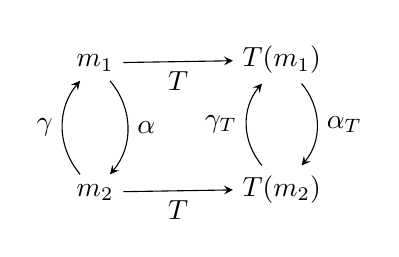
\begin{tikzpicture}
  \matrix (m) [matrix of math nodes,row sep=3em,column sep=4em,minimum width=2em]
  {
     m_1 & T(m_1) \\
     m_2 & T(m_2) \\
  };
  \path[-stealth]
    (m-1-1) edge [bend left=40] node [right] {$\alpha$}   (m-2-1)
            edge                node [below] {$T$}        (m-1-2)
    (m-2-1) edge [bend left=40] node [left]  {$\gamma$}   (m-1-1)
            edge                node [below] {$T$}        (m-2-2)
    (m-1-2) edge [bend left=40] node [right] {$\alpha_T$} (m-2-2)
    (m-2-2) edge [bend left=40] node [left]  {$\gamma_T$} (m-1-2)
  ;
\end{tikzpicture}
\end{center}

\item 

It transports mappings to an executable transition system, that is there
exists $ \Pi $ s.t. for all monads $m$ and functors $ \Sigma $,
$( \alpha   \rightarrow  m( \beta ))  \galois{\alpha}{\gamma}  ( \Sigma ( \alpha )  \rightarrow         \Sigma ( \beta ))$
implies
$( \alpha   \rightarrow  T(m)( \beta ))  \galois{\alpha}{\gamma}  ( \Pi ( \Sigma )( \alpha )  \rightarrow   \Pi ( \Sigma )( \beta ))$.

\begin{center}
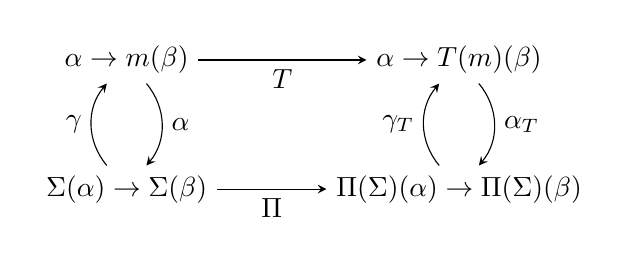
\begin{tikzpicture}
  \matrix (m) [matrix of math nodes,row sep=3em,column sep=4em,minimum width=2em]
  {
             \alpha \rightarrow m(\beta)      & \alpha              \rightarrow T(m)(\beta)        \\
     \Sigma(\alpha) \rightarrow \Sigma(\beta) & \Pi(\Sigma)(\alpha) \rightarrow \Pi(\Sigma)(\beta) \\
  };
  \path[-stealth]
    (m-1-1) edge [bend left=40] node [right] {$\alpha$}   (m-2-1)
            edge                node [below] {$T$}        (m-1-2)
    (m-2-1) edge [bend left=40] node [left]  {$\gamma$}   (m-1-1)
            edge                node [below] {$\Pi$}      (m-2-2)
    (m-1-2) edge [bend left=40] node [right] {$\alpha_T$} (m-2-2)
    (m-2-2) edge [bend left=40] node [left]  {$\gamma_T$} (m-1-2)
  ;
\end{tikzpicture}
\end{center}

\end{enumerate} \end{definition} Property (1) transports Galois
connections between monads, and property (2) transports Galois
connections between transition systems. By composing the 2-dimensional
diagrams (1) and (2) into a 3-dimensional diagram (which we do not show)
we establish the following theorem: \begin{theorem} If $T$ is a Galois
transformer, then it is sufficient to prove that underlying monads
$m _1 $ and $m _2 $ form a Galois connection
$m _1   \galois{\alpha}{\gamma}  m _2 $ in order to establish
$ \Pi ( \Sigma  _1 )  \galois{\alpha}{\gamma}   \Pi ( \Sigma  _2 )$.
\label{galois-theorem} \end{theorem} This is the workhorse of our entire
proof framework, allowing us to reason about monadic actions, like the
monadic interpreter $ \itop{step} $ from section \ref{the-interpreter},
and derive properties about the induced transition system, which is how
the analysis is executed, for free. \begin{proposition}
$S _t  \lbrack s \rbrack $, $FS _t  \lbrack s \rbrack $ and
$ \mathcal{P}  _t $ are Galois transformers. \end{proposition} The
proofs are sketched earlier in Section
\ref{a-compositional-monadic-framework}.

\par

\subsection{Building Transformer
Stacks}\label{building-transformer-stacks}

\par

We can now build monad transformer stacks from combinations of
$S _t  \lbrack s \rbrack $, $FS \lbrack s \rbrack  _t $ and
$ \mathcal{P}  _t $ which automatically construct the following
properties:

\par

\begin{itemize}
\itemsep1pt\parskip0pt\parsep0pt
\item
  The resulting monad has the combined effects of all pieces of the
  transformer stack.
\item
  Actions in the resulting monad map to a state space transition system
  $ \Sigma   \rightarrow   \Sigma $ for some $ \Sigma $, allowing one to
  execute the analysis.
\item
  Galois connections between $ \Concrete{\Sigma} $ and
  $ \Abstract{\Sigma} $ are established piecewise from monad transformer
  components.
\end{itemize}

\par

We instantiate our interpreter to the following monad stacks in
decreasing order of precision:

\par

\vspace{4pt}

\small\begin{tabular}{ >{$}l<{$} | >{$}l<{$} | >{$}l<{$} }

S _t   \lbrack \Abstract{\litEnv} \rbrack       & S _t   \lbrack \Abstract{\litEnv} \rbrack        & S _t   \lbrack \Abstract{\litEnv} \rbrack      \\
S _t   \lbrack \Abstract{\litKAddr} \rbrack     & S _t   \lbrack \Abstract{\litKAddr} \rbrack      & S _t   \lbrack \Abstract{\litKAddr} \rbrack    \\
S _t   \lbrack \Abstract{\litKStore} \rbrack    & S _t   \lbrack \Abstract{\litKStore} \rbrack     & S _t   \lbrack \Abstract{\litKStore} \rbrack   \\
S _t   \lbrack \Abstract{\litTime} \rbrack      & S _t   \lbrack \Abstract{\litTime} \rbrack       & S _t   \lbrack \Abstract{\litTime} \rbrack     \\
S _t   \lbrack \Abstract{\litStore} \rbrack     &               &  \mathcal{P}  _t           \\
 \mathcal{P}  _t            & FS _t   \lbrack \Abstract{\litStore} \rbrack     & S _t   \lbrack \Abstract{\litStore} \rbrack    \\

\end{tabular}\normalsize \vspace{4pt}

\par

\noindent
From left to right these give path-sensitive, flow-sensitive and
flow-insensitive analyses for the data-store.

\par

Another benefit of our approach is that we can easily select different
path and flow sensitivity properties for the data-store and stack-store
independent of each other, merely by rearranging the order of
composition.

\par

\vspace{8pt}

\small\begin{tabular}{ >{$}l<{$} | >{$}l<{$} | >{$}l<{$} }

S _t   \lbrack \Abstract{\litEnv} \rbrack       & S _t   \lbrack \Abstract{\litEnv} \rbrack        & S _t   \lbrack \Abstract{\litEnv} \rbrack      \\
S _t   \lbrack \Abstract{\litKAddr} \rbrack     & S _t   \lbrack \Abstract{\litKAddr} \rbrack      & S _t   \lbrack \Abstract{\litKAddr} \rbrack    \\
S _t   \lbrack \Abstract{\litTime} \rbrack      & S _t   \lbrack \Abstract{\litTime} \rbrack       & S _t   \lbrack \Abstract{\litTime} \rbrack     \\
S _t   \lbrack \Abstract{\litKStore} \rbrack    &               &  \mathcal{P}  _t           \\
 \mathcal{P}  _t            & FS _t   \lbrack \Abstract{\litKStore} \rbrack    & S _t   \lbrack \Abstract{\litKStore} \rbrack   \\
S _t   \lbrack \Abstract{\litStore} \rbrack     & S _t   \lbrack \Abstract{\litStore} \rbrack      & S _t   \lbrack \Abstract{\litStore} \rbrack    \\

\end{tabular}\normalsize \vspace{8pt}

\par

\noindent
From left to right these give analysis which are all flow-insensitive in
the data-store, but path-sensitive, flow-sensitive and flow-insensitive
in the stack-store.

\par

\section{Implementation}\label{implementation-1}

\par

We have implemented our framework in Haskell and applied it to compute
analyses for $ \ttbfop{\lambda{}IF} $. Our implementation provides path
sensitivity, flow sensitivity, and flow insensitivity as a
semantics-independent monad library. The code shares a striking
resemblance with the math.

\par

Our implementation is suitable for prototyping and exploring the design
space of static analyzers. Our analyzer supports exponentially more
compositions of analysis features than any current analyzer. For
example, our implementation is the first which can combine arbitrary
choices in call-site, object, path and flow sensitivities. Furthermore,
the user can choose different path and flow sensitivities for each
component of the state space.

\par

Our implementation {\tt maam} supports command-line flags for garbage
collection, mCFA, call-site sensitivity, object sensitivity, and path
and flow sensitivity.

{\small\tt
\par \noindent ./maam prog.lam --gc --mcfa --kcfa=1 --ocfa=2
\par \noindent \hspace{2em} --data-store=flow-sen --stack-store=path-sen
}
\par \noindent

These flags are implemented completely independently of one another and
their combination is applied to a single parameterized monadic
interpreter. Furthermore, using Galois transformers allows us to prove
each combination correct in one fell swoop.

\par

A developer wishing to use our library to develop analyzers for their
language of choice inherits as much of the analysis infrastructure as
possible. We provide call-site, object, path and flow sensitivities as
language-independent libraries. To support analysis for a new language a
developer need only implement:

\par

\begin{itemize}
\itemsep1pt\parskip0pt\parsep0pt
\item
  A monadic semantics for their language, using state and nondeterminism
  effects.
\item
  The abstract value domain, and optionally the concrete value domain if
  they wish to recover concrete execution.
\item
  Intentional optimizations for their semantics like garbage collection
  and mcfa.
\end{itemize}

\par

The developer then receives the following for free through our analysis
library:

\par

\begin{itemize}
\itemsep1pt\parskip0pt\parsep0pt
\item
  A family of monads which implement their effect interface and give
  different path and flow sensitivities.
\item
  An execution engine for each monad to drive the analysis.
\item
  Mechanisms for call-site and object sensitivities.
\end{itemize}

\par

Not only is a developer able to reuse our implementation of call-site,
object, path and flow sensitivities, they need not understand the
execution machinery or soundness proofs for them either. They need only
verify that their monadic semantics is monotonic w.r.t. the analysis
parameters, and that their abstract value domain forms a Galois
connection. The execution and correctness of the final analyzer is
constructed automatically given these two properties.

\par

Our implementation is publicly available and can be installed as a cabal
package: {\small\tt cabal install maam}.

\par

\section{Related Work}\label{related-work}

\par

\paragraph{Overview}

\par

Program analysis comes in many forms such as points-to
\cite{dvanhorn:Andersen1994Program}, flow
\cite{dvanhorn:Jones:1981:LambdaFlow}, or shape analysis
\cite{dvanhorn:Chase1990Analysis}, and the literature is vast. (See
\citet{dvanhorn:hind-paste01,dvanhorn:Midtgaard2012Controlflow} for
surveys.) Much of the research has focused on developing families or
frameworks of analyses that endow the abstraction with a number of
knobs, levers, and dials to tune precision and compute efficiently (some
examples include
\citet{dvanhorn:Shivers:1991:CFA, dvanhorn:nielson-nielson-popl97,
dvanhorn:Milanova2005Parameterized, davdar:van-horn:2010:aam}; there are
many more). These parameters come in various forms with overloaded
meanings such as object \cite{dvanhorn:Milanova2005Parameterized,
dvanhorn:Smaragdakis2011Pick}, context
\cite{dvanhorn:Sharir:Interprocedural,
dvanhorn:Shivers:1991:CFA}, path \cite{davdar:das:2002:esp}, and heap
\cite{davdar:van-horn:2010:aam} sensitivities, or some combination
thereof \cite{dvanhorn:Kastrinis2013Hybrid}.

\par

These various forms can all be cast in the theory of abstraction
interpretation of \citet{dvanhorn:Cousot:1977:AI,
dvanhorn:Cousot1979Systematic} and understood as computable
approximations of an underlying concrete interpreter. Our work
demonstrates that if this underlying concrete interpreter is written in
monadic style, monad transformers are a useful way to organize and
compose these various kinds of program abstractions in a modular and
language-independent way.

\par

This work is inspired by the trifecta combination of
\citeauthor{dvanhorn:Cousot:1977:AI}'s theory of abstract interpretation
based on Galois connections \cite{dvanhorn:Cousot:1977:AI,
dvanhorn:Cousot1979Systematic, dvanhorn:Cousot98-5},
\citeauthor{davdar:Moggi:1989:Monads}'s original monad transformers
\cite{davdar:Moggi:1989:Monads} which were later popularized in
\citeauthor{dvanhorn:Liang1995Monad}'s \emph{Monad Transformers and
Modular Interpreters} \cite{dvanhorn:Liang1995Monad}, and
\citeauthor{dvanhorn:Sergey2013Monadic}'s \emph{Monadic Abstract
Interpreters} \cite{dvanhorn:Sergey2013Monadic}.

\par

\par

\citet{dvanhorn:Liang1995Monad} first demonstrated how monad
transformers could be used to define building blocks for constructing
(concrete) interpreters. Their interpreter monad
\mbox{\(\mathit{InterpM}\)} bears a strong resemblance to ours. We show
this ``building blocks'' approach to interpreter construction also
extends to \emph{abstract} interpreter construction using Galois
transformers. Moreover, we show that these monad transformers can be
proved sound via a Galois connection to their concrete counterparts,
ensuring the soundness of any stack built from sound blocks of Galois
transformers. Soundness proofs of various forms of analysis are
notoriously brittle with respect to language and analysis features. A
reusable framework of Galois transformers offers a potential way forward
for a modular metatheory of program analysis.

\par

\citet{dvanhorn:Cousot98-5} develops a ``calculational approach'' to
analysis design whereby analyses are not designed and then verified
\emph{post facto}, but rather derived by positing an abstraction and
calculating it from the concrete interpreter using Galois connections.
These calculations are done by hand. Our approach offers a limited
ability to automate the calculation process by relying on monad
transformers to combine different abstractions.

\par

We build directly on the work of Abstracting Abstract Machines (AAM) by
\citet{davdar:van-horn:2010:aam} and
\citet{dvanhorn:Smaragdakis2011Pick} in our parameterization of abstract
time to achieve call-site and object sensitivity. More notably, we
follow the AAM philosophy of instrumenting a concrete semantics
\emph{first} and performing a systematic abstraction \emph{second}. This
greatly simplifies the Galois connection arguments during systematic
abstraction. However, this is at the added cost of proving that the
instrumented semantics simulate the original concrete semantics.

\par

\paragraph{Monadic Abstract Interpreters}

\par

\citeauthor{dvanhorn:Sergey2013Monadic} first introduced the concept of
writing abstract interpreters in monadic style in \emph{Monadic Abstract
Interpreters} (MAI)\cite{dvanhorn:Sergey2013Monadic}, in which
variations in analysis are also recovered through new monad
implementations. However, our approach is considerably different from
MAI.

\par

In MAI, the framework's interface is based on \emph{denotation
functions} for every syntactic form of the language (See
``CPSInterface'', Figure 2 in MAI). This design decision has far
reaching consequences for the entire approach. The denotation functions
in MAI are language-specific and specialized to their example language.
MAI uses a single monad stack fixed to the denotation function
interface: state on top of list (Section 5.3.1 in MAI). New analyses are
achieved through multiple denotation functions into this single monad.
Analyses in MAI are all fixed to be path-sensitive, and the methodology
for incorporating other path or flow properties is to surgically
instrument the execution of the analysis with a custom Galois connection
(Section 6.5 in MAI). Lastly, the framework provides no reasoning
principles or proofs of soundness for the denotation function interface.
\emph{A user of MAI must inline the definitions of each analysis and
prove their implementation correct from scratch each time.}

\par

By contrast, our framework's interface is based on state and
nondeterminism \emph{monadic effects} (Section
\ref{the-analysis-monad}). This interface comes equipped with reasoning
principles, allowing one to verify the correctness of a monadic
interpreter \emph{independent of a particular monad}, which is not
possible in MAI. State and nondeterminism monadic effects capture the
essence of \emph{small-step relational semantics}, and are therefore
truly language independent. Our tools are reusable for any semantics
described as a small-step state machine relation. Because we place the
monadic interpreter behind an interface of effects rather than
denotation functions, we are able to introduce language-independent
monads which capture flow-sensitivity and flow-insensitivity (Sections
\ref{varying-path-and-flow-sensitivity} and
\ref{a-compositional-monadic-framework}), and we show how to compose
these features with other analysis design choices (Sections
\ref{analysis-parameters} and \ref{a-compositional-monadic-framework}).
The monadic effect interface also allows us to separate the monad from
the abstract domain, both of which are tightly coupled in MAI. Finally,
our framework is compositional through the use of monad transformers
(Section \ref{a-compositional-monadic-framework}) which construct
execution engines and proofs of soundness for free.

\par

We do not achieve correctness and compositionality \emph{in addition} to
our transition from denotation functions to monadic effects; rather we
achieve correctness and compositionality \emph{through it}; such a
transition is essential, primary and novel to our work.

\par

\paragraph{Widening for Control-Flow}

\par

\citeauthor{dvanhorn:Hardekopf2014Widening} also introduce a unifying
account of control flow properties in \emph{Widening for Control-Flow}
(WCF)\cite{dvanhorn:Hardekopf2014Widening}, accounting for path, flow
and call-site sensitivities . WCF achieves this through an
instrumentation of the abstract machine's state space which is allowed
to track arbitrary contextual information, up to the path-history of the
entire execution. WCF also develops a modular proof framework, proving
the bulk of soundness proofs for each instantiation of the
instrumentation at once.

\par

Our work achieves similar goals, although isolating path and flow
sensitivity is not our primary objective. While WCF is based on a
language-dependent instrumentation of the semantics, we achieve
variations in path and flow sensitivity by modifying
language-independent control properties of the interpreter through a
monad.

\par

Particular strengths of WCF are the wide range of choices for
control-flow sensitivity which are shown to be implementable within the
design, and the modular proof framework. For example, WCF is able to
also account for call-site sensitivity through their design; we must
account for call-site sensitivity through a different mechanism.

\par

Particular strengths of our work is the understanding of path and flow
sensitivity not through instrumentation but through control properties
of the interpreter, and also a modular proof framework, although modular
in a different sense from WCF. We also show how to compose different
path and flow sensitivity choices for independent components of the
state space, like a flow-sensitive data-store and path-sensitive
stack-store, for example.

\par

\section{Conclusion}\label{conclusion}

\par

We have shown that \emph{Galois transformers}, monad transformers that
transport (1) Galois connections and (2) mappings to an executable
transition system, are effective, language-independent building blocks
for constructing program analyzers, and form the basis of a modular,
reusable and composable metatheory for program analysis.

\par

In the end, we hope language independent characterizations of analysis
ingredients will both facilitate the systematic construction of program
analyses and bridge the gap between various communities which often work
in isolation.


% \appendix
% \section{Appendix Title}
% 
% Appendix body.
% 
% \acks
% 
% Acknowledgments body.

\balance
\bibliographystyle{abbrvnat}
\bibliography{dvanhorn,davdar}

\appendix
\section{PLDI 2015 Summary review}

This paper was previously submitted to PLDI 2015. It advanced through
the first round with favorable reviews, but received a short negative
review in the second round stating ``this paper seems like a rather
straightforward and not very deep extension of the PLDI'13 paper on
monadic abstract interpreters.''

The summary review of the PC discussion stated:

\begin{quote}
There was extensive discussion of this paper at the PC meeting, with
arguments on both sides. From the perspective of the functional
programming experts, there is only a small increment from the previous
PLDI'13 paper---moving from monads to monad transformers is a
seemingly obvious step with little novelty. From the perspective of
the static analysis experts, the paper presents a very interesting
view on how to structure abstract interpreters that shows how to apply
existing work in the functional world to static analysis. Ultimately
we looked at the section on Galois transfomers (sic) as the point of
potential novelty from the functional perspective, and found that
there was too little there to convince people that Galois transformers
are a non-trivial variation of monad transformers. We encourage the
authors to continue this work and to try and clarify the novelty from
the functional perspective (or target the paper more closely to the
static analysis community). We also encourage the authors to work on
the exposition in the paper to make it more accessible.
\end{quote}

The present version of this paper has aimed to clarify the novelty of
this work and explain how, while the idea of ``going from monads to
monad transformers'' is in some sense an obvious idea, there is no way
to get there from the PLDI'13 paper of Sergey et al., without
significant research.  That research is the subject of this paper.

We have also incorporated all of the feedback toward making the paper
more accessible.

For completeness, we include our response to the claim ``this paper
seems like a rather straightforward and not very deep extension of the
PLDI'13 paper on monadic abstract interpreters.''  Much of this
content has been incorporated into the paper.

\begin{quote}
We respectfully disagree with this assessment of the paper. Let us clarify the
relationship with Sergey et al \cite{dvanhorn:Sergey2013Monadic} (PLDI'13).

The primary contributions of Sergey et al are:

\begin{itemize}
\item Monads can serve as a good organizational mechanism for constructing abstract
  interpreters.
\item Different monads can be used to describe a wide range of abstract
  interpreters.
\end{itemize}

In our view, shortcomings of Sergey et al are:

\begin{itemize}
\item No restrictions are placed on the monads used, allowing for
  absurd and unsound analyses.

\item There is no soundness framework for the approach. Instantiated
  analyses must be reasoned about on an ad-hoc basis after inlining
  the abstractions.

\item The monads are not compositional or reusable across languages as
  claimed in the paper.
\end{itemize}

Our paper remedies these shortcomings:

\begin{itemize}
\item Our interface between interpreters and monads is well-defined
  and based on language-independent monadic effects, allowing one to
  reason on both sides of the interface.

\item Our framework constructs end-to-end Galois connections for
  proofs of soundness.

\item Monads in our framework can be defined and proved correct
independently of a particular language.  Furthermore, constructing a
new large monad in our framework is a simple composition of the monad
transformers described in the paper.
\end{itemize}

In addition to these improvements, our paper has the following
desirable properties:

\begin{itemize}
\item In our framework, intentional analysis optimizations like abstract garbage
  collection and shape analysis can be defined and proven correct for all
  concrete and abstract interpreters at once (for a particular language).

\item Our framework fully compartmentalizes the choice of control sensitivity for the
  analysis.
\end{itemize}

Alternatively, our paper can be seen as an extension of Liang et al
\cite{dvanhorn:Liang1995Monad} applied to abstract interpreters rather
than standard interpreters. We believe this is a deep insight into the
theory of monad transformers and modular interpreters not present in
Sergey et al.
\end{quote}

\end{document}
